\chapter{Supplementary Information to \Chapref{effectivepopsize}}

\section{Supplementary Tables}

1-8


\section{Supplementary Figures}




\begin{figure}[h!]
\centering
\makebox[\textwidth]{
        \includegraphics[width=0.4\linewidth]{Figures/SuppFigures/FigureS1_Demog.pdf}}
\caption[Range of incorrect source populations provided in the island model scenarios.]{Range of incorrect source populations provided in the island model scenarios for estimates from \textsc{mlne}. Grayed out arrows indicate the true immigration source to the focal patch while dotted lines indicate the incorrectly assumed source of immigration. For the stepping stone IBD model, the related patch used was one separated from the focal patch by three or thirteen intervening patches, with no other cases tested.}
\label{fig:supp_demog}
\end{figure}


\begin{figure}[h!]
\centering
\makebox[\textwidth]{
        \includegraphics[width=1.2\linewidth]{Figures/SuppFigures/SuppFigS2__PropInf.pdf}}
\caption[Proportion of estimates that reported infinite values of $N_e$.]{Proportion of estimates that reported infinite values of $N_e$. The proportions are out of 100 replicates except in cases where methods were not run for the full 100 replicates or the result was considered invalid as stated by the program output or described by the program author(s). Note from the main text that negative values produced from \textsc{neestimator} have been counted as infinites, as per the recommendation of the authors \citep{Do:2014}, and that for \textsc{mlne}'s likelihood estimate, an estimate at the upper bound of the prior $N_e$ is also considered as infinite here.}
\label{fig:supp_propinf}
\end{figure}


\begin{landscape}


\begin{figure}[h!]
\centering
\makebox[\textwidth]{
        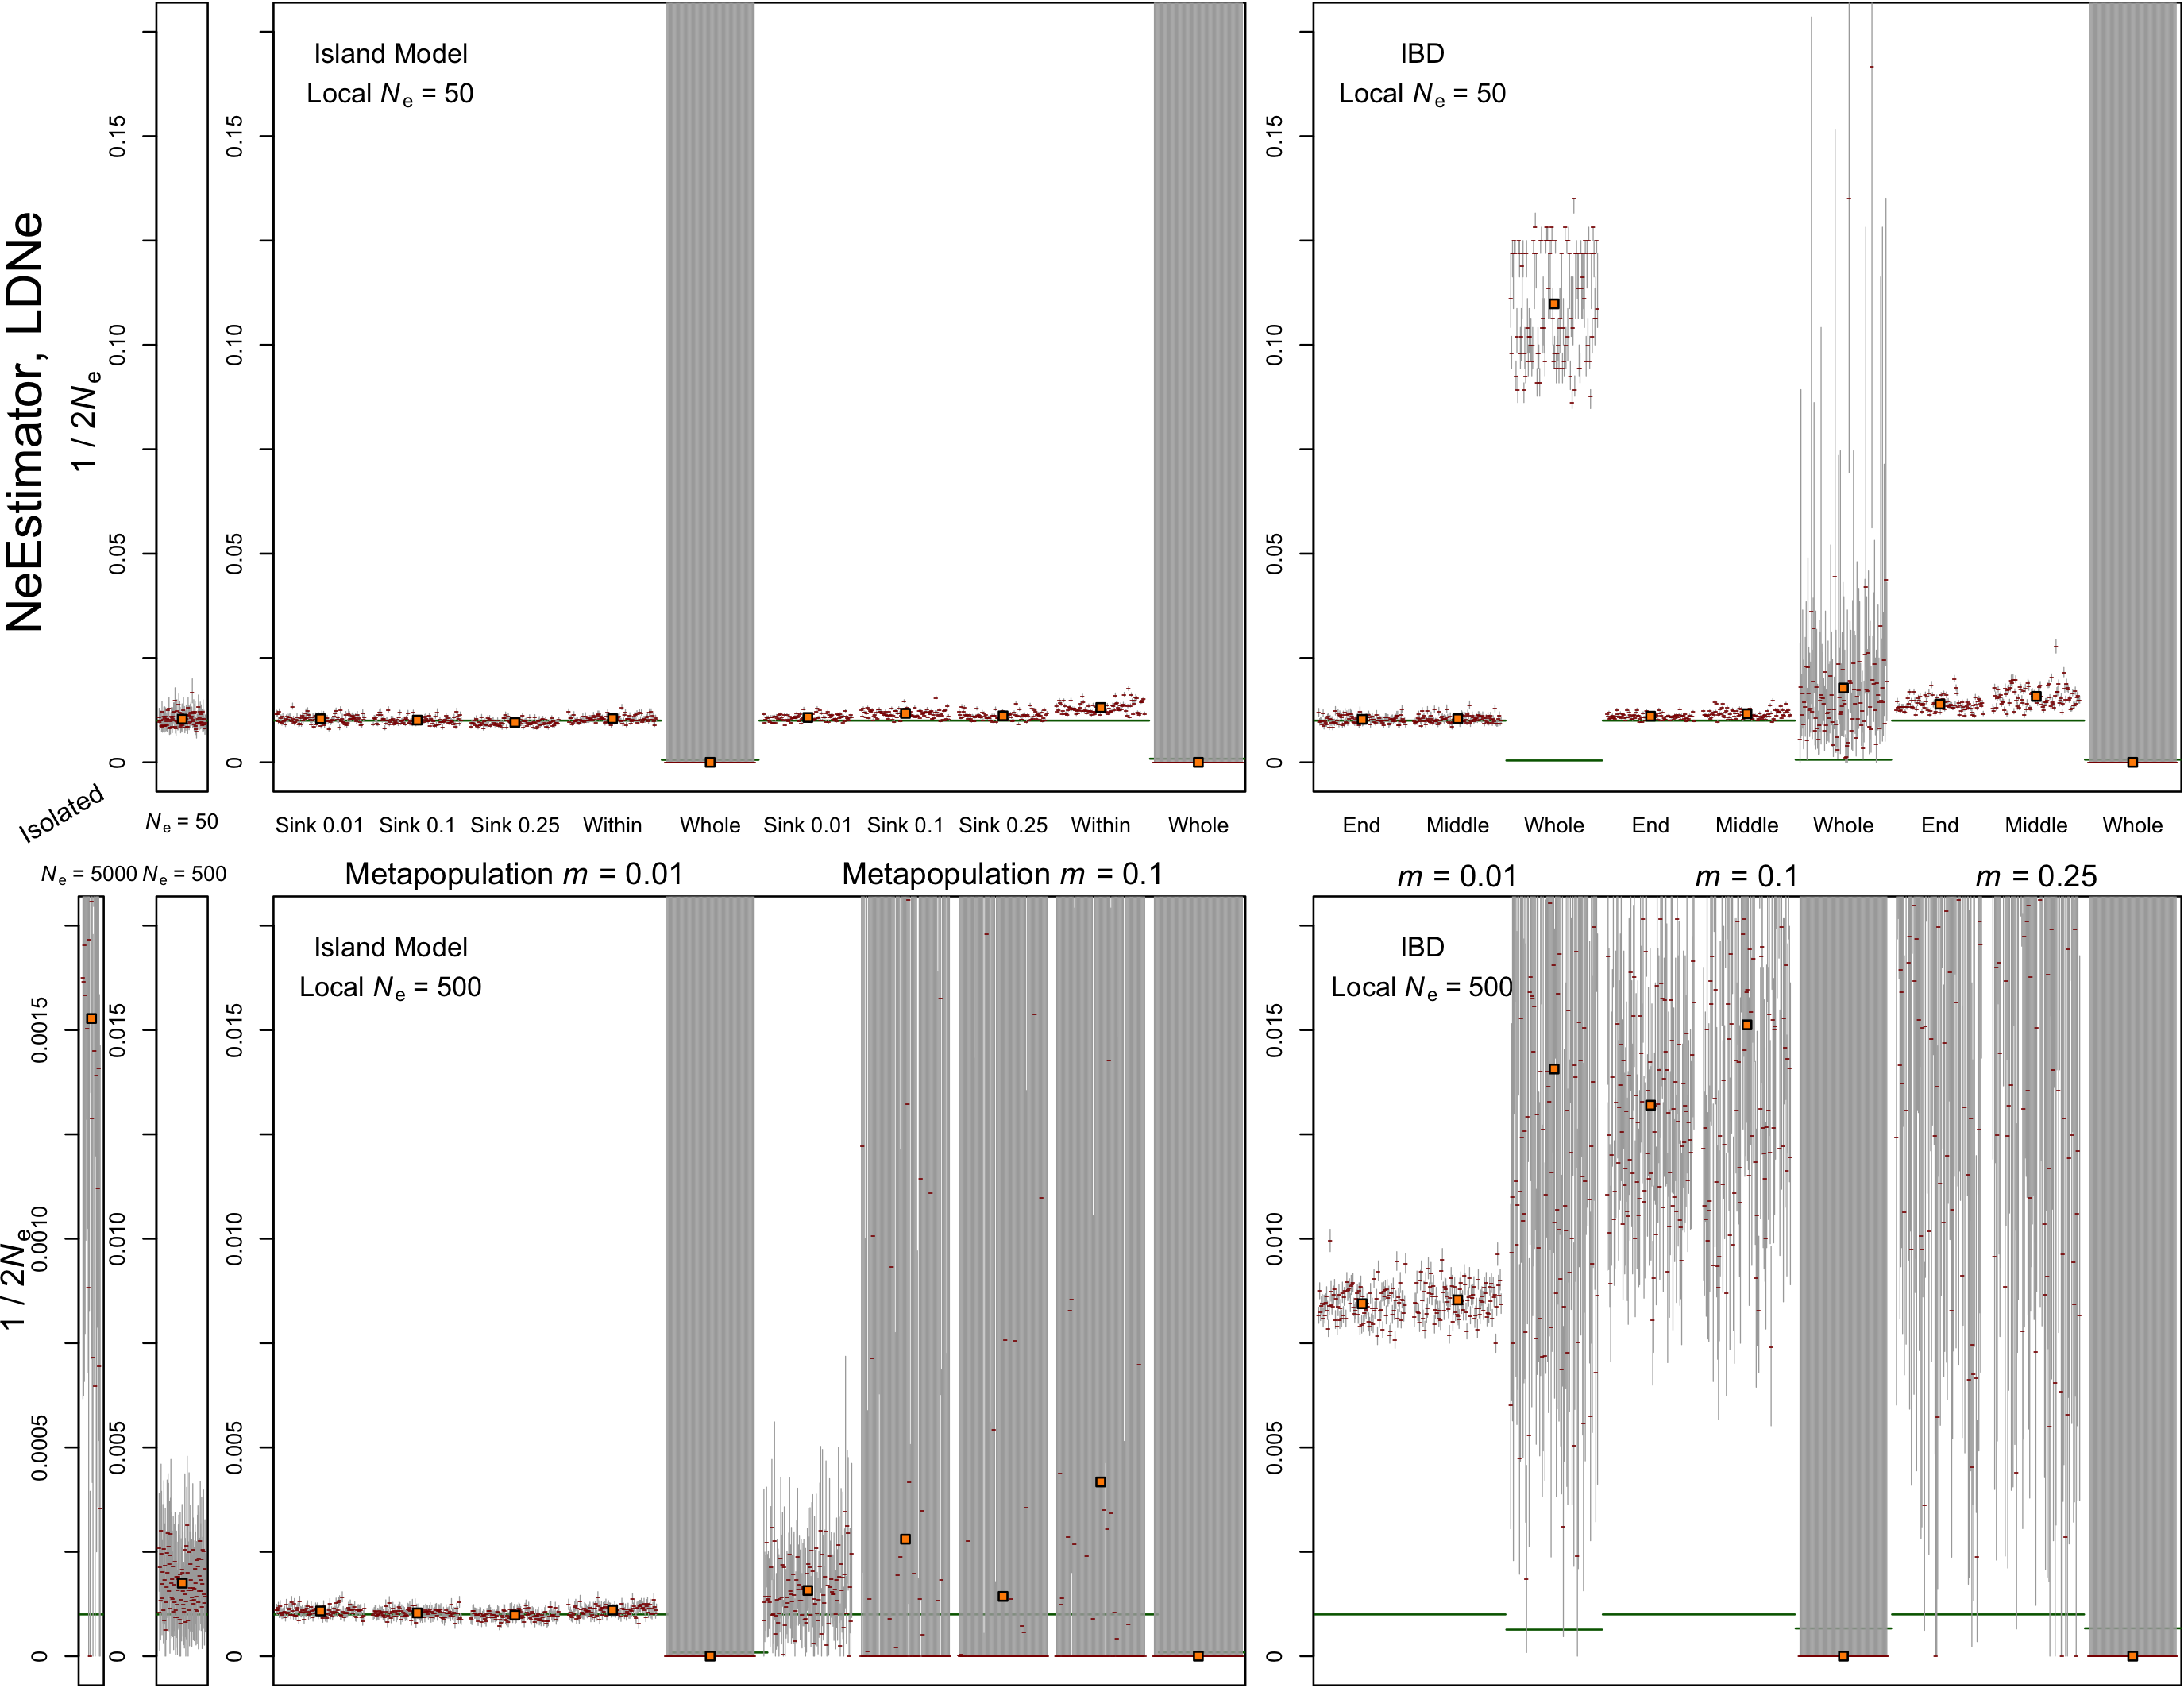
\includegraphics[width=1\linewidth]{Figures/SuppFigures/FigureS2__LDNeRawResults.png}}
\caption[All replicate estimated $N_e$ values for \textsc{neestimator}'s \textsc{ldne} method across all scenarios..]{All replicate estimated $N_e$ values for \textsc{neestimator}'s \textsc{ldne} method across all scenarios. True $N_e$ is shown by the horizontal green lines, point estimates in red with their average indicate by the orange square, and $95\%$ confidence intervals by gray vertical lines. $y$-axis is $\frac{1}{2 N_e}$ and scenarios are shown across the $x$-axis, labeled in the center row. The three isolated, no migration cases are shown on the left, followed by the island model migration cases in the middle and the stepping stone IBD cases on the right, with $N_e = 50$ along the top row and 500 along the bottom row.}
\label{fig:supp_ldne}
\end{figure}

\begin{figure}[h!]
\centering
\makebox[\textwidth]{
        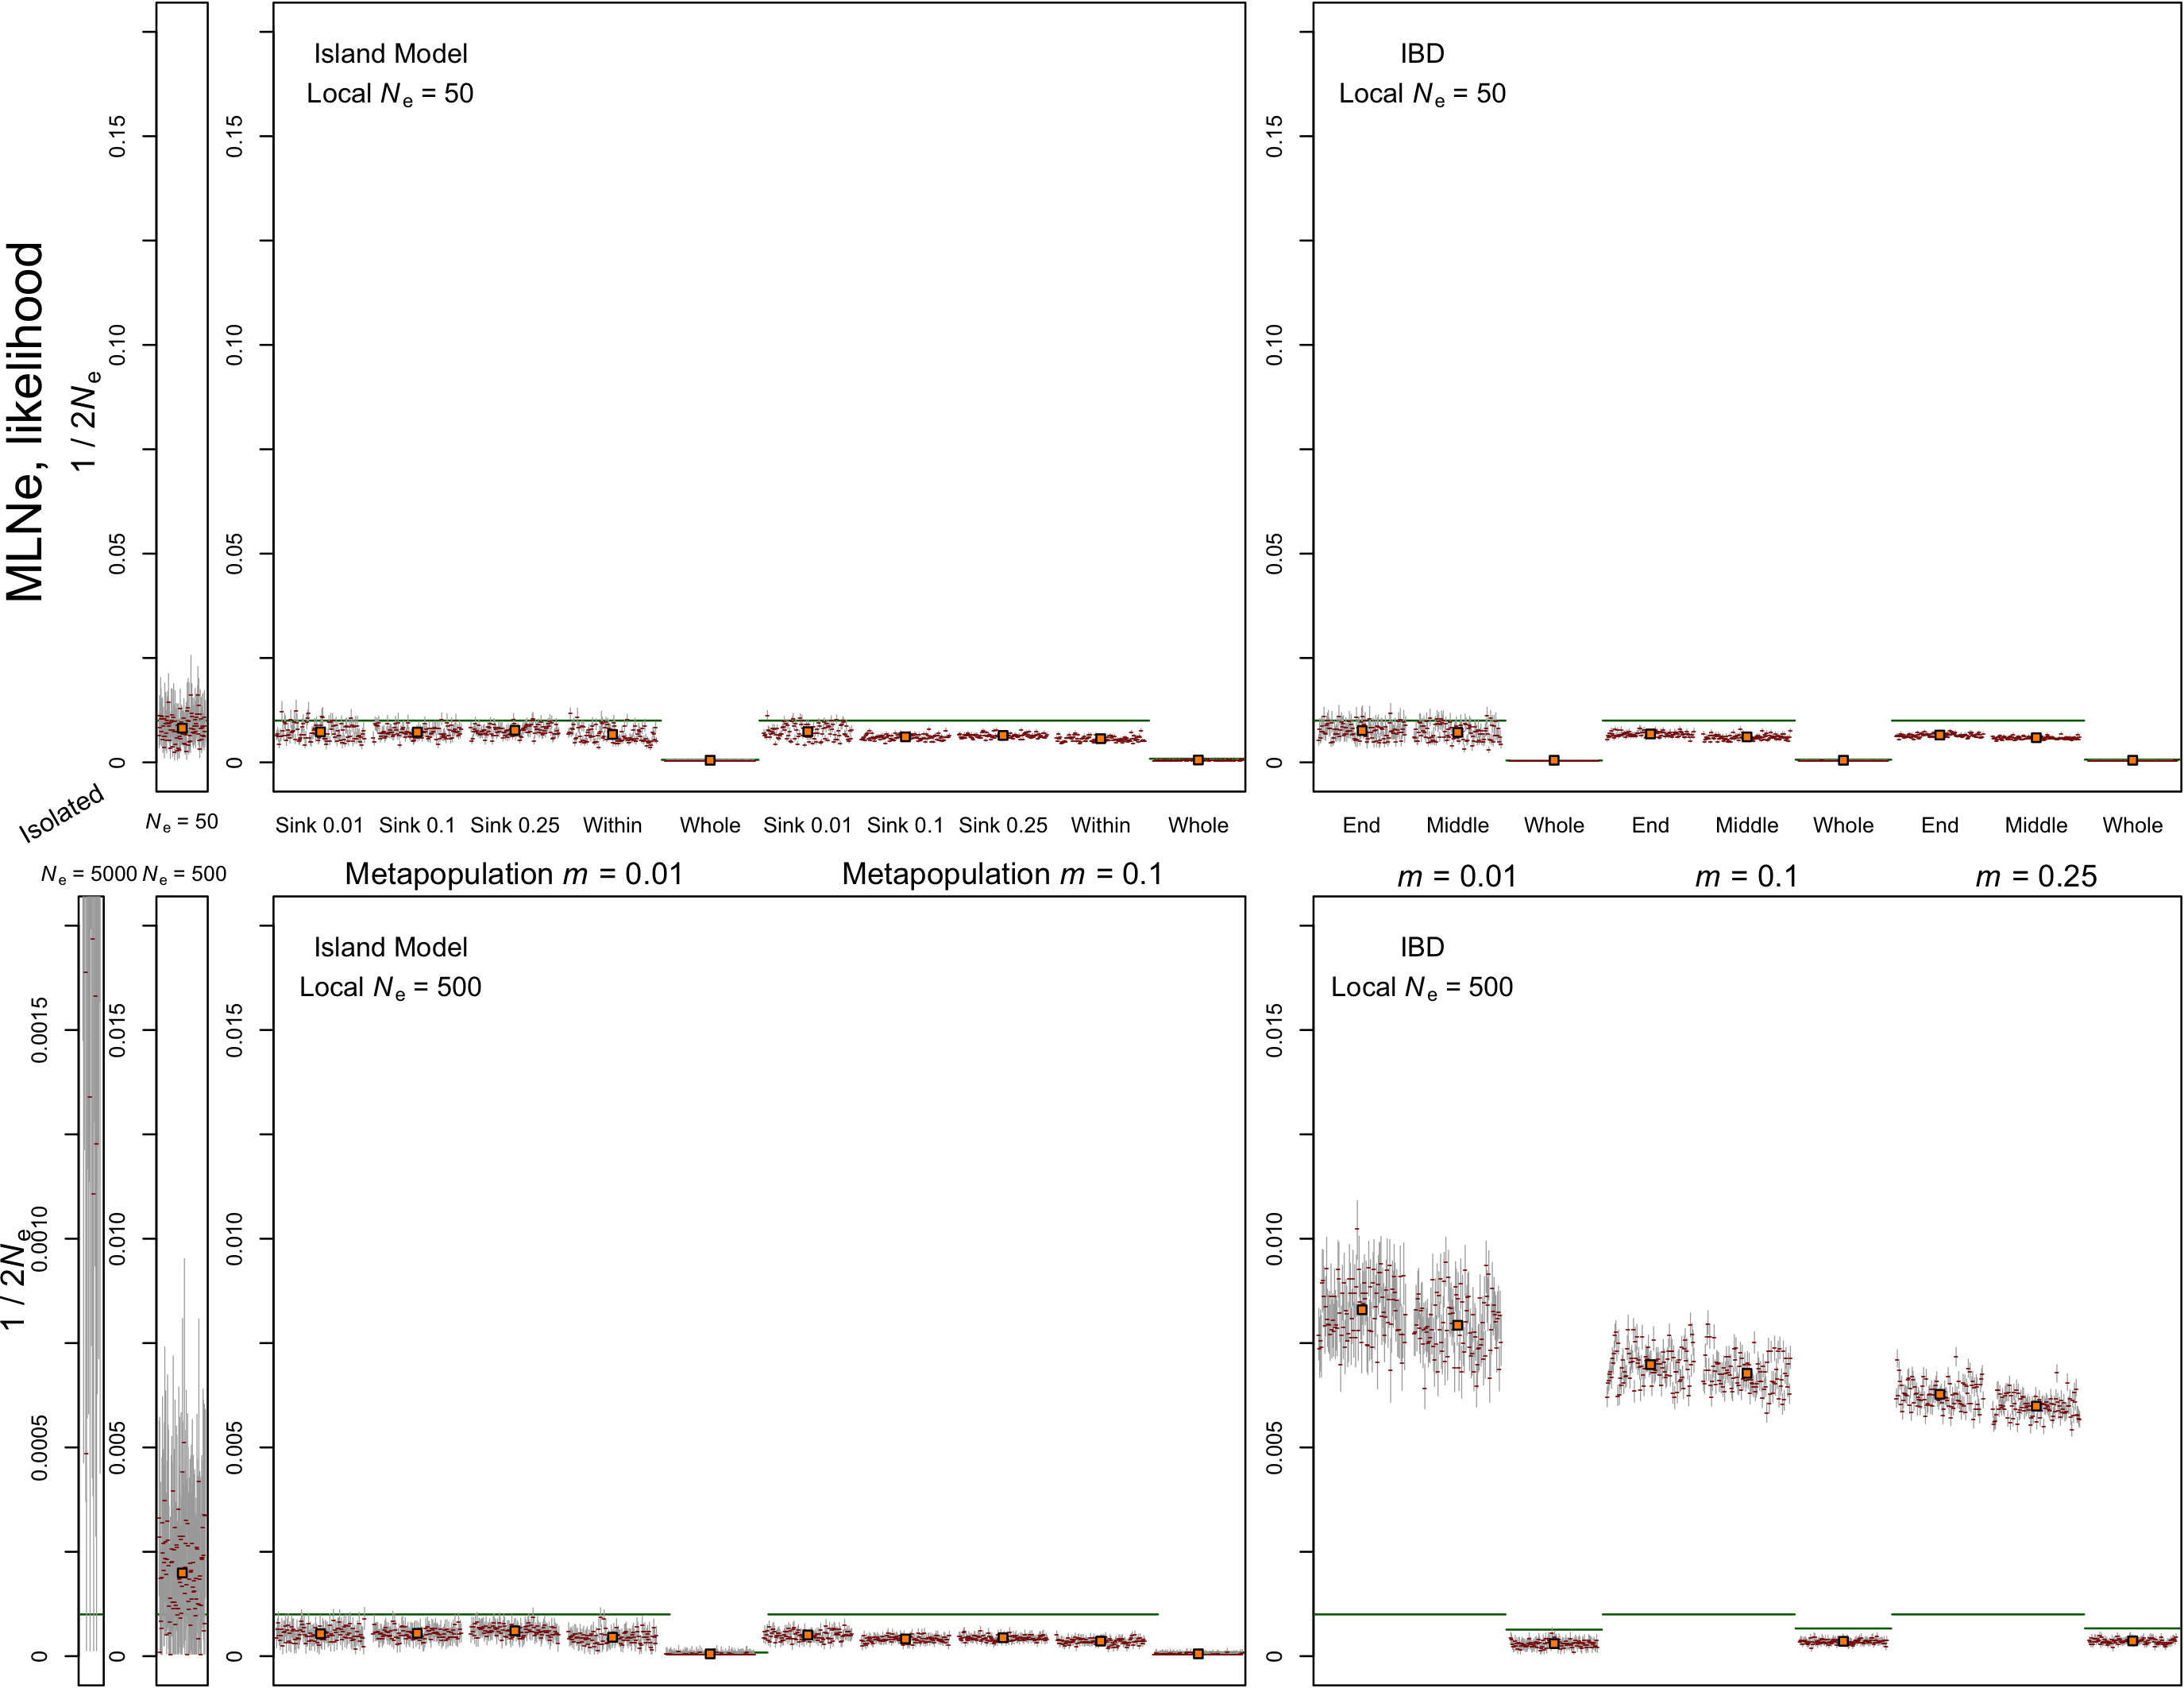
\includegraphics[width=0.8\linewidth]{Figures/SuppFigures/FigureS3a__MLNeLikRawResults.png}}
\caption[All replicate estimated $N_e$ values for \textsc{mlne} likelihood method across all scenarios.]{All replicate estimated $N_e$ values for \textsc{mlne} likelihood method across all scenarios. True $N_e$ is shown by the horizontal green lines, point estimates in red with their average indicate by the orange square, and $95\%$ confidence intervals by gray vertical lines. $y$-axis is $\frac{1}{2 N_e}$ and scenarios are shown across the $x$-axis, labeled in the center row. The three isolated, no migration cases are shown on the left, followed by the island model migration cases in the middle and the stepping stone IBD cases on the right, with $N_e = 50$ along the top row and 500 along the bottom row.}
\label{fig:supp_mlnelik}
\end{figure}


\begin{figure}[h!]
\centering
\makebox[\textwidth]{
        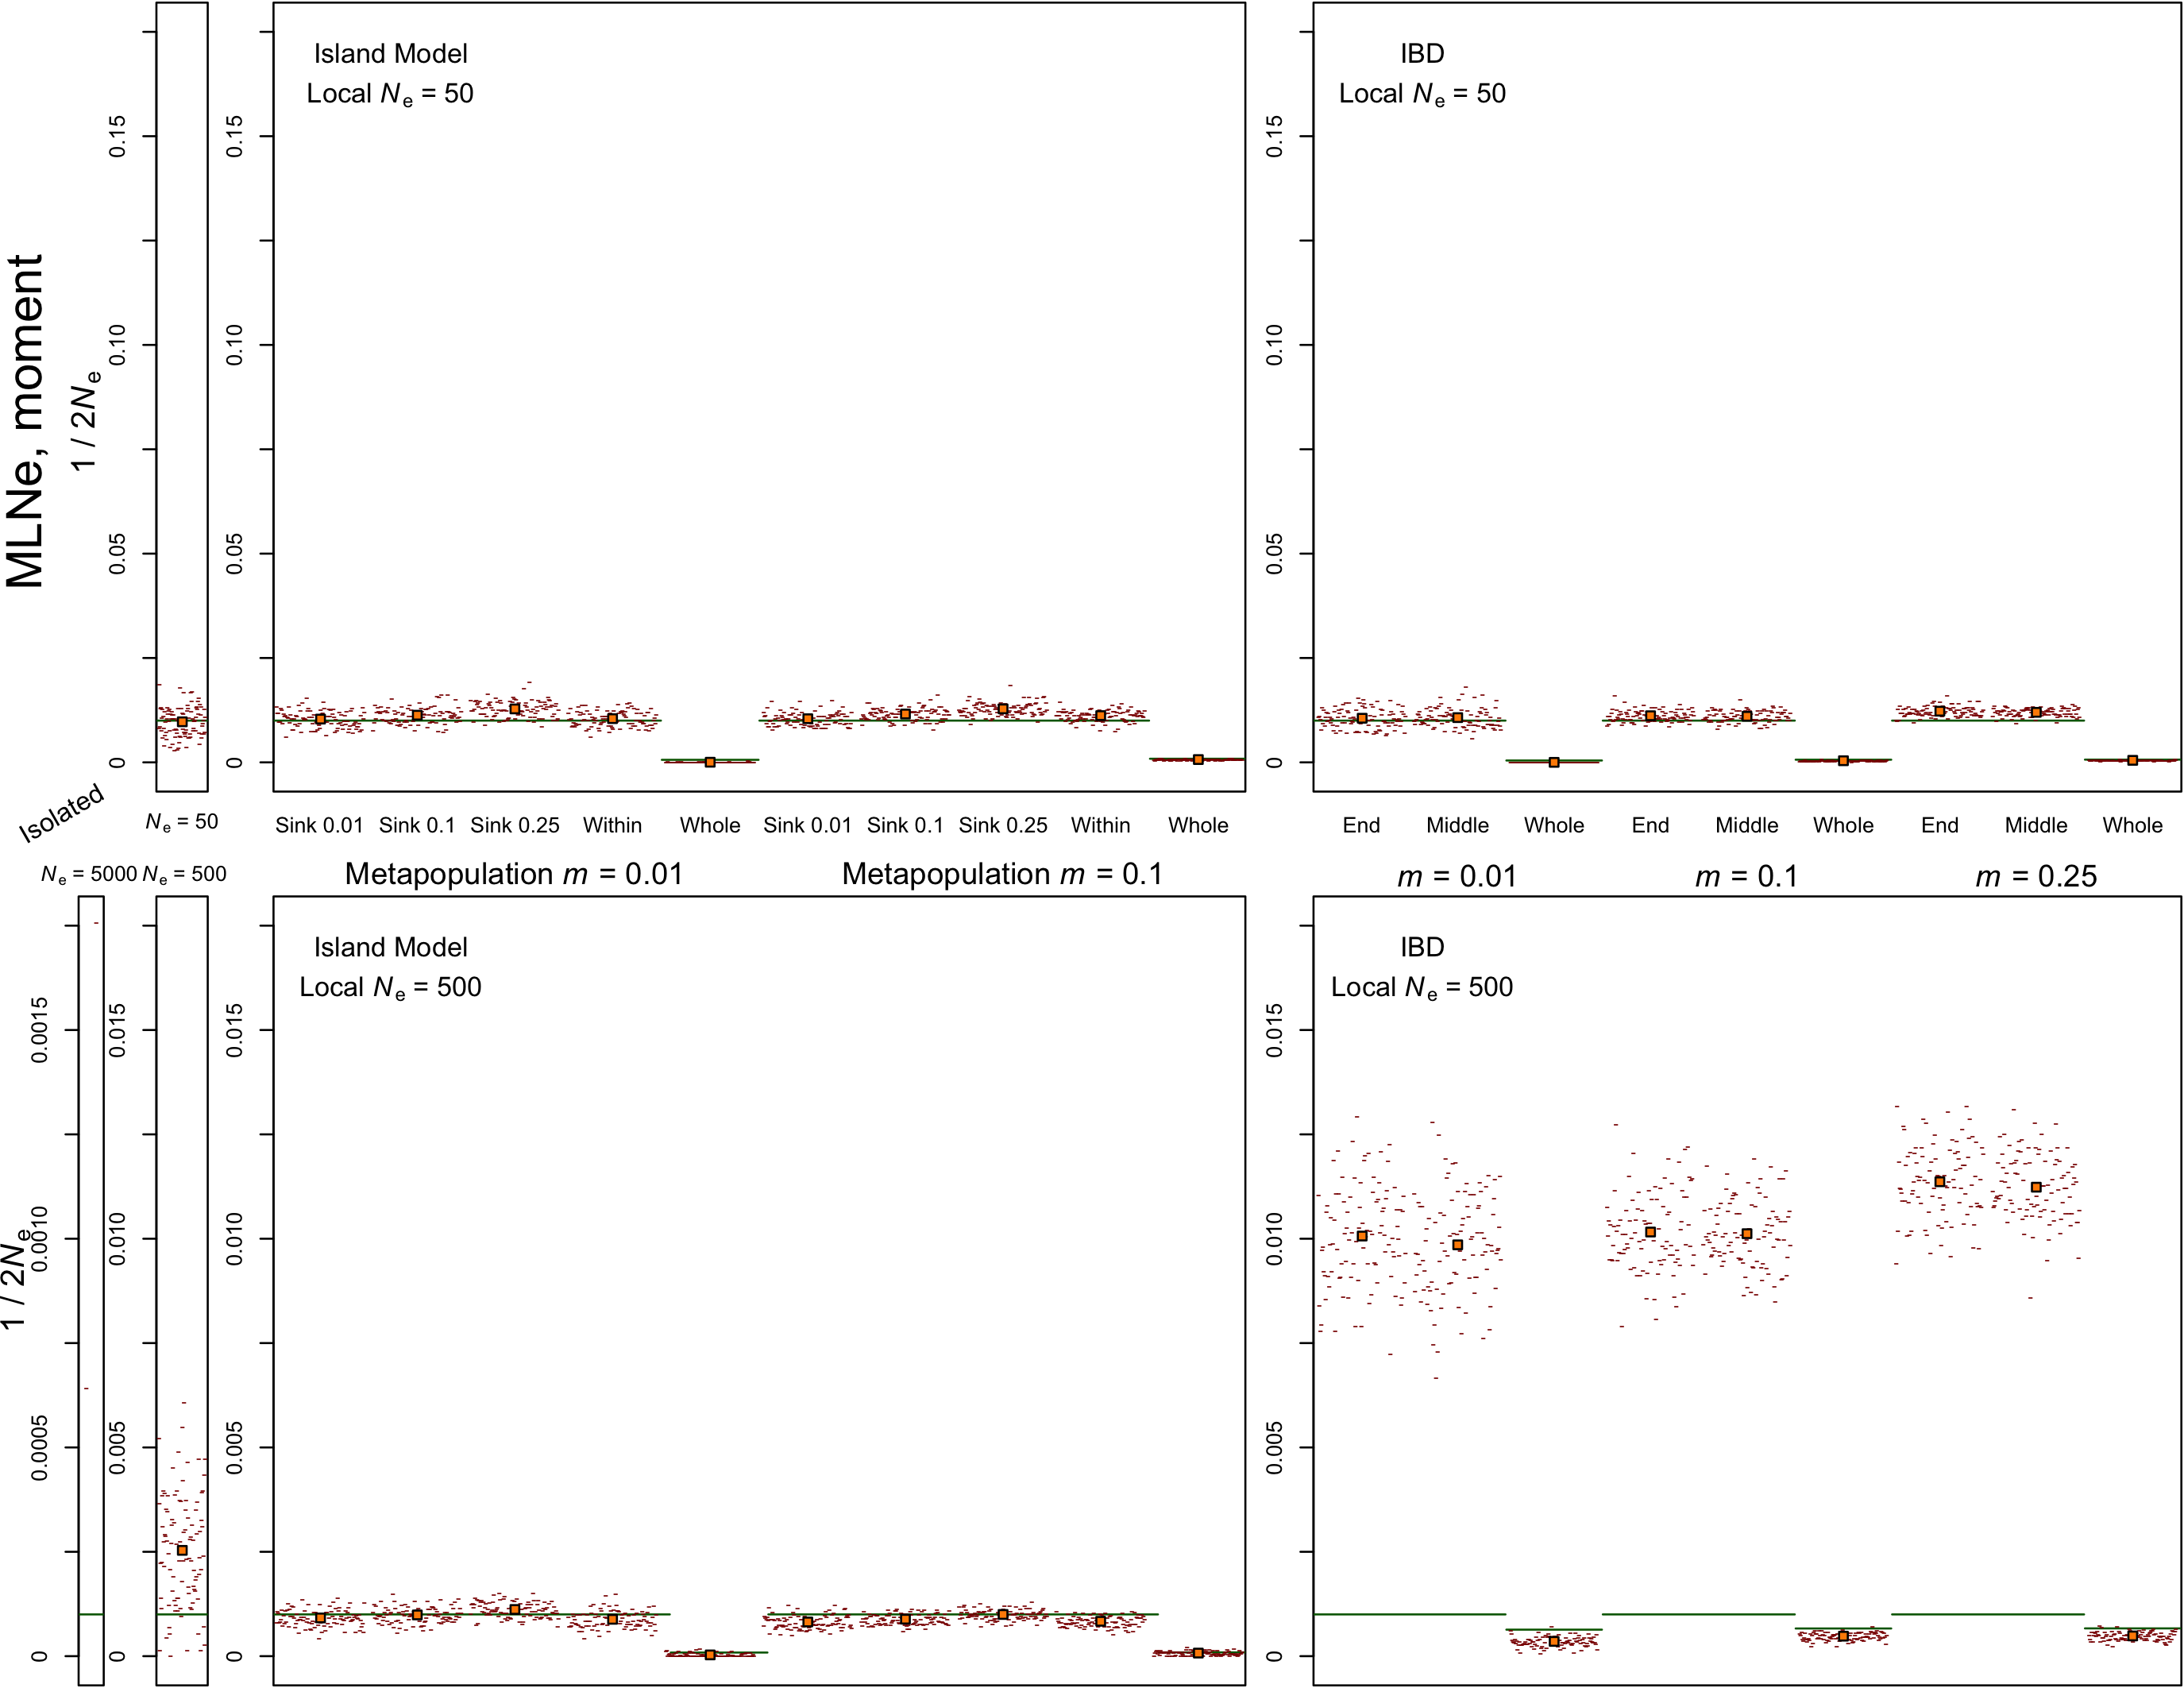
\includegraphics[width=0.8\linewidth]{Figures/SuppFigures/FigureS3b__MLNeMomRawResults.png}}
\caption[All replicate estimated $N_e$ values for \textsc{mlne} moment method across all scenarios.]{All replicate estimated $N_e$ values for \textsc{mlne} moment method across all scenarios. True $N_e$ is shown by the horizontal green lines and point estimates in red with their average indicate by the orange square. Note that the moment estimate does not produce confidence intervals. $y$-axis is $\frac{1}{2 N_e}$ and scenarios are shown across the $x$-axis, labeled in the center row. The three isolated, no migration cases are shown on the left, followed by the island model migration cases in the middle and the stepping stone IBD cases on the right, with $N_e = 50$ along the top row and 500 along the bottom row.}
\label{fig:supp_mlnemom}
\end{figure}


\begin{figure}[h!]
\centering
\makebox[\textwidth]{
        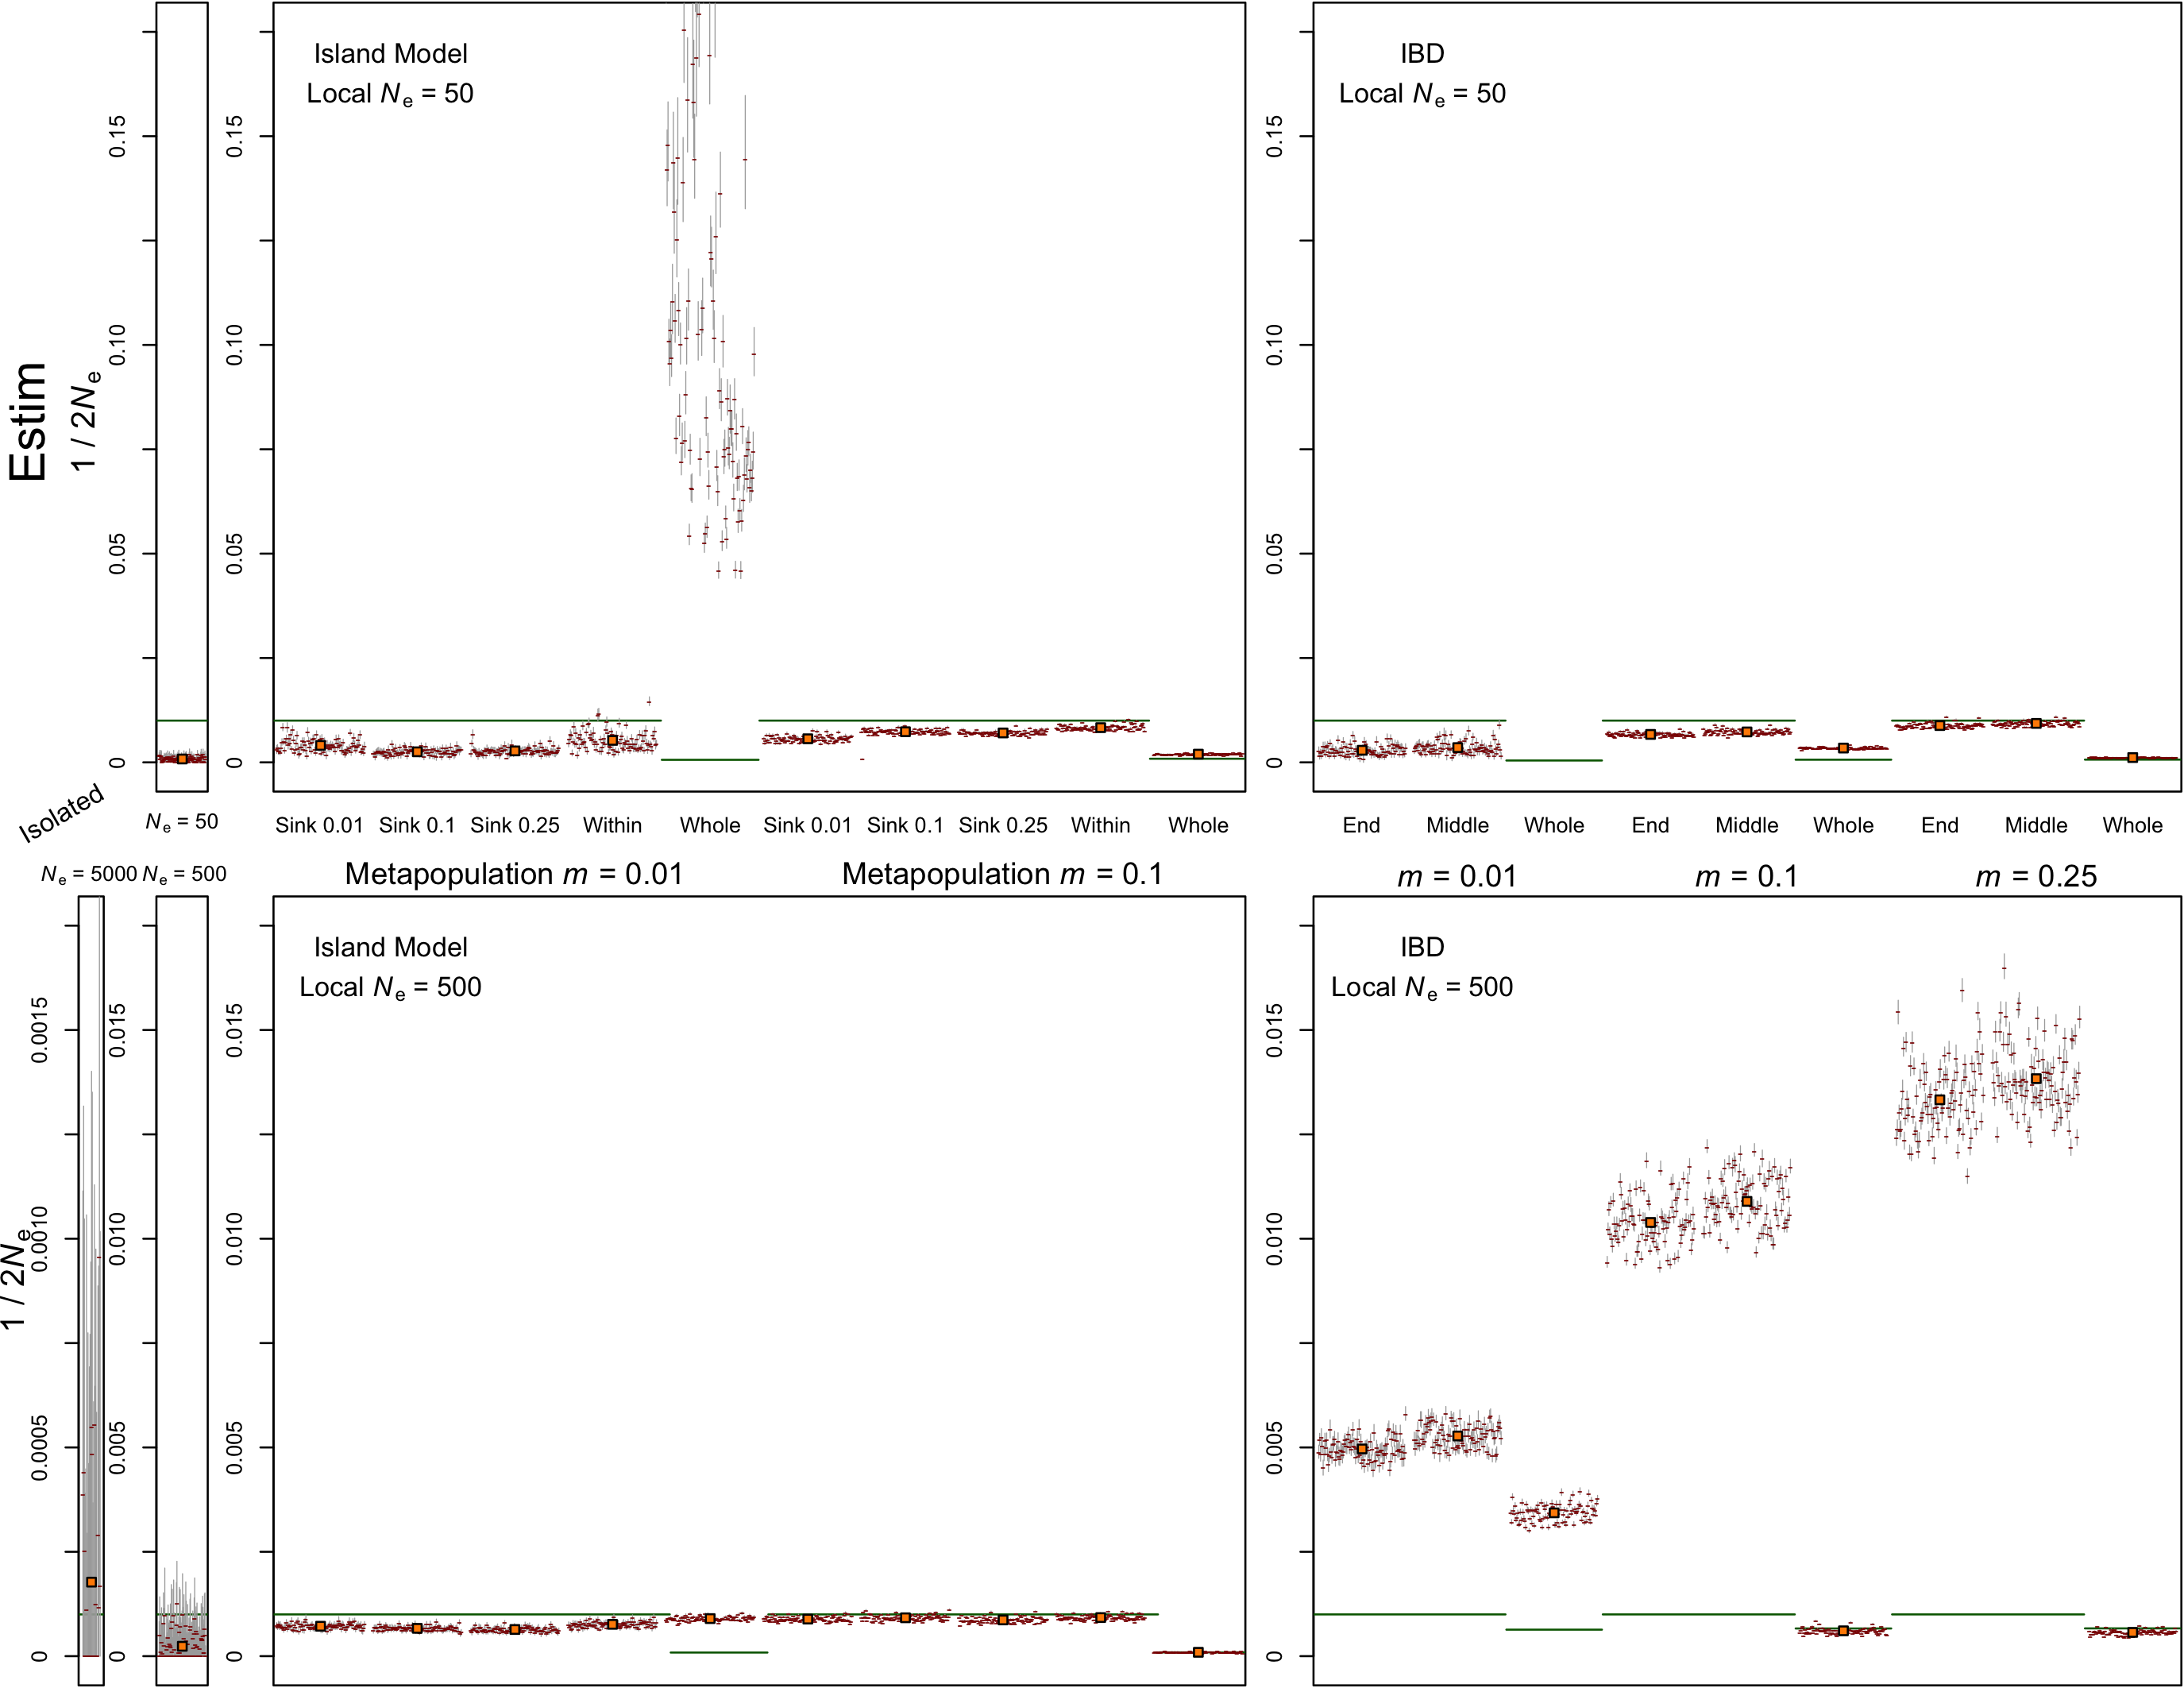
\includegraphics[width=0.8\linewidth]{Figures/SuppFigures/FigureS4__EstimRawResults.png}}
\caption[All replicate estimated $N_e$ values for \textsc{estim} across all scenarios.]{All replicate estimated $N_e$ values for \textsc{estim} across all scenarios. True $N_e$ is shown by the horizontal green lines, point estimates in red with their average indicate by the orange square, and $95\%$ confidence intervals by gray vertical lines. $y$-axis is $\frac{1}{2 N_e}$ and scenarios are shown across the $x$-axis, labeled in the center row. The three isolated, no migration cases are shown on the left, followed by the island model migration cases in the middle and the stepping stone IBD cases on the right, with $N_e = 50$ along the top row and 500 along the bottom row.}
\label{fig:supp_estim}
\end{figure}


\begin{figure}[h!]
\centering
\makebox[\textwidth]{
        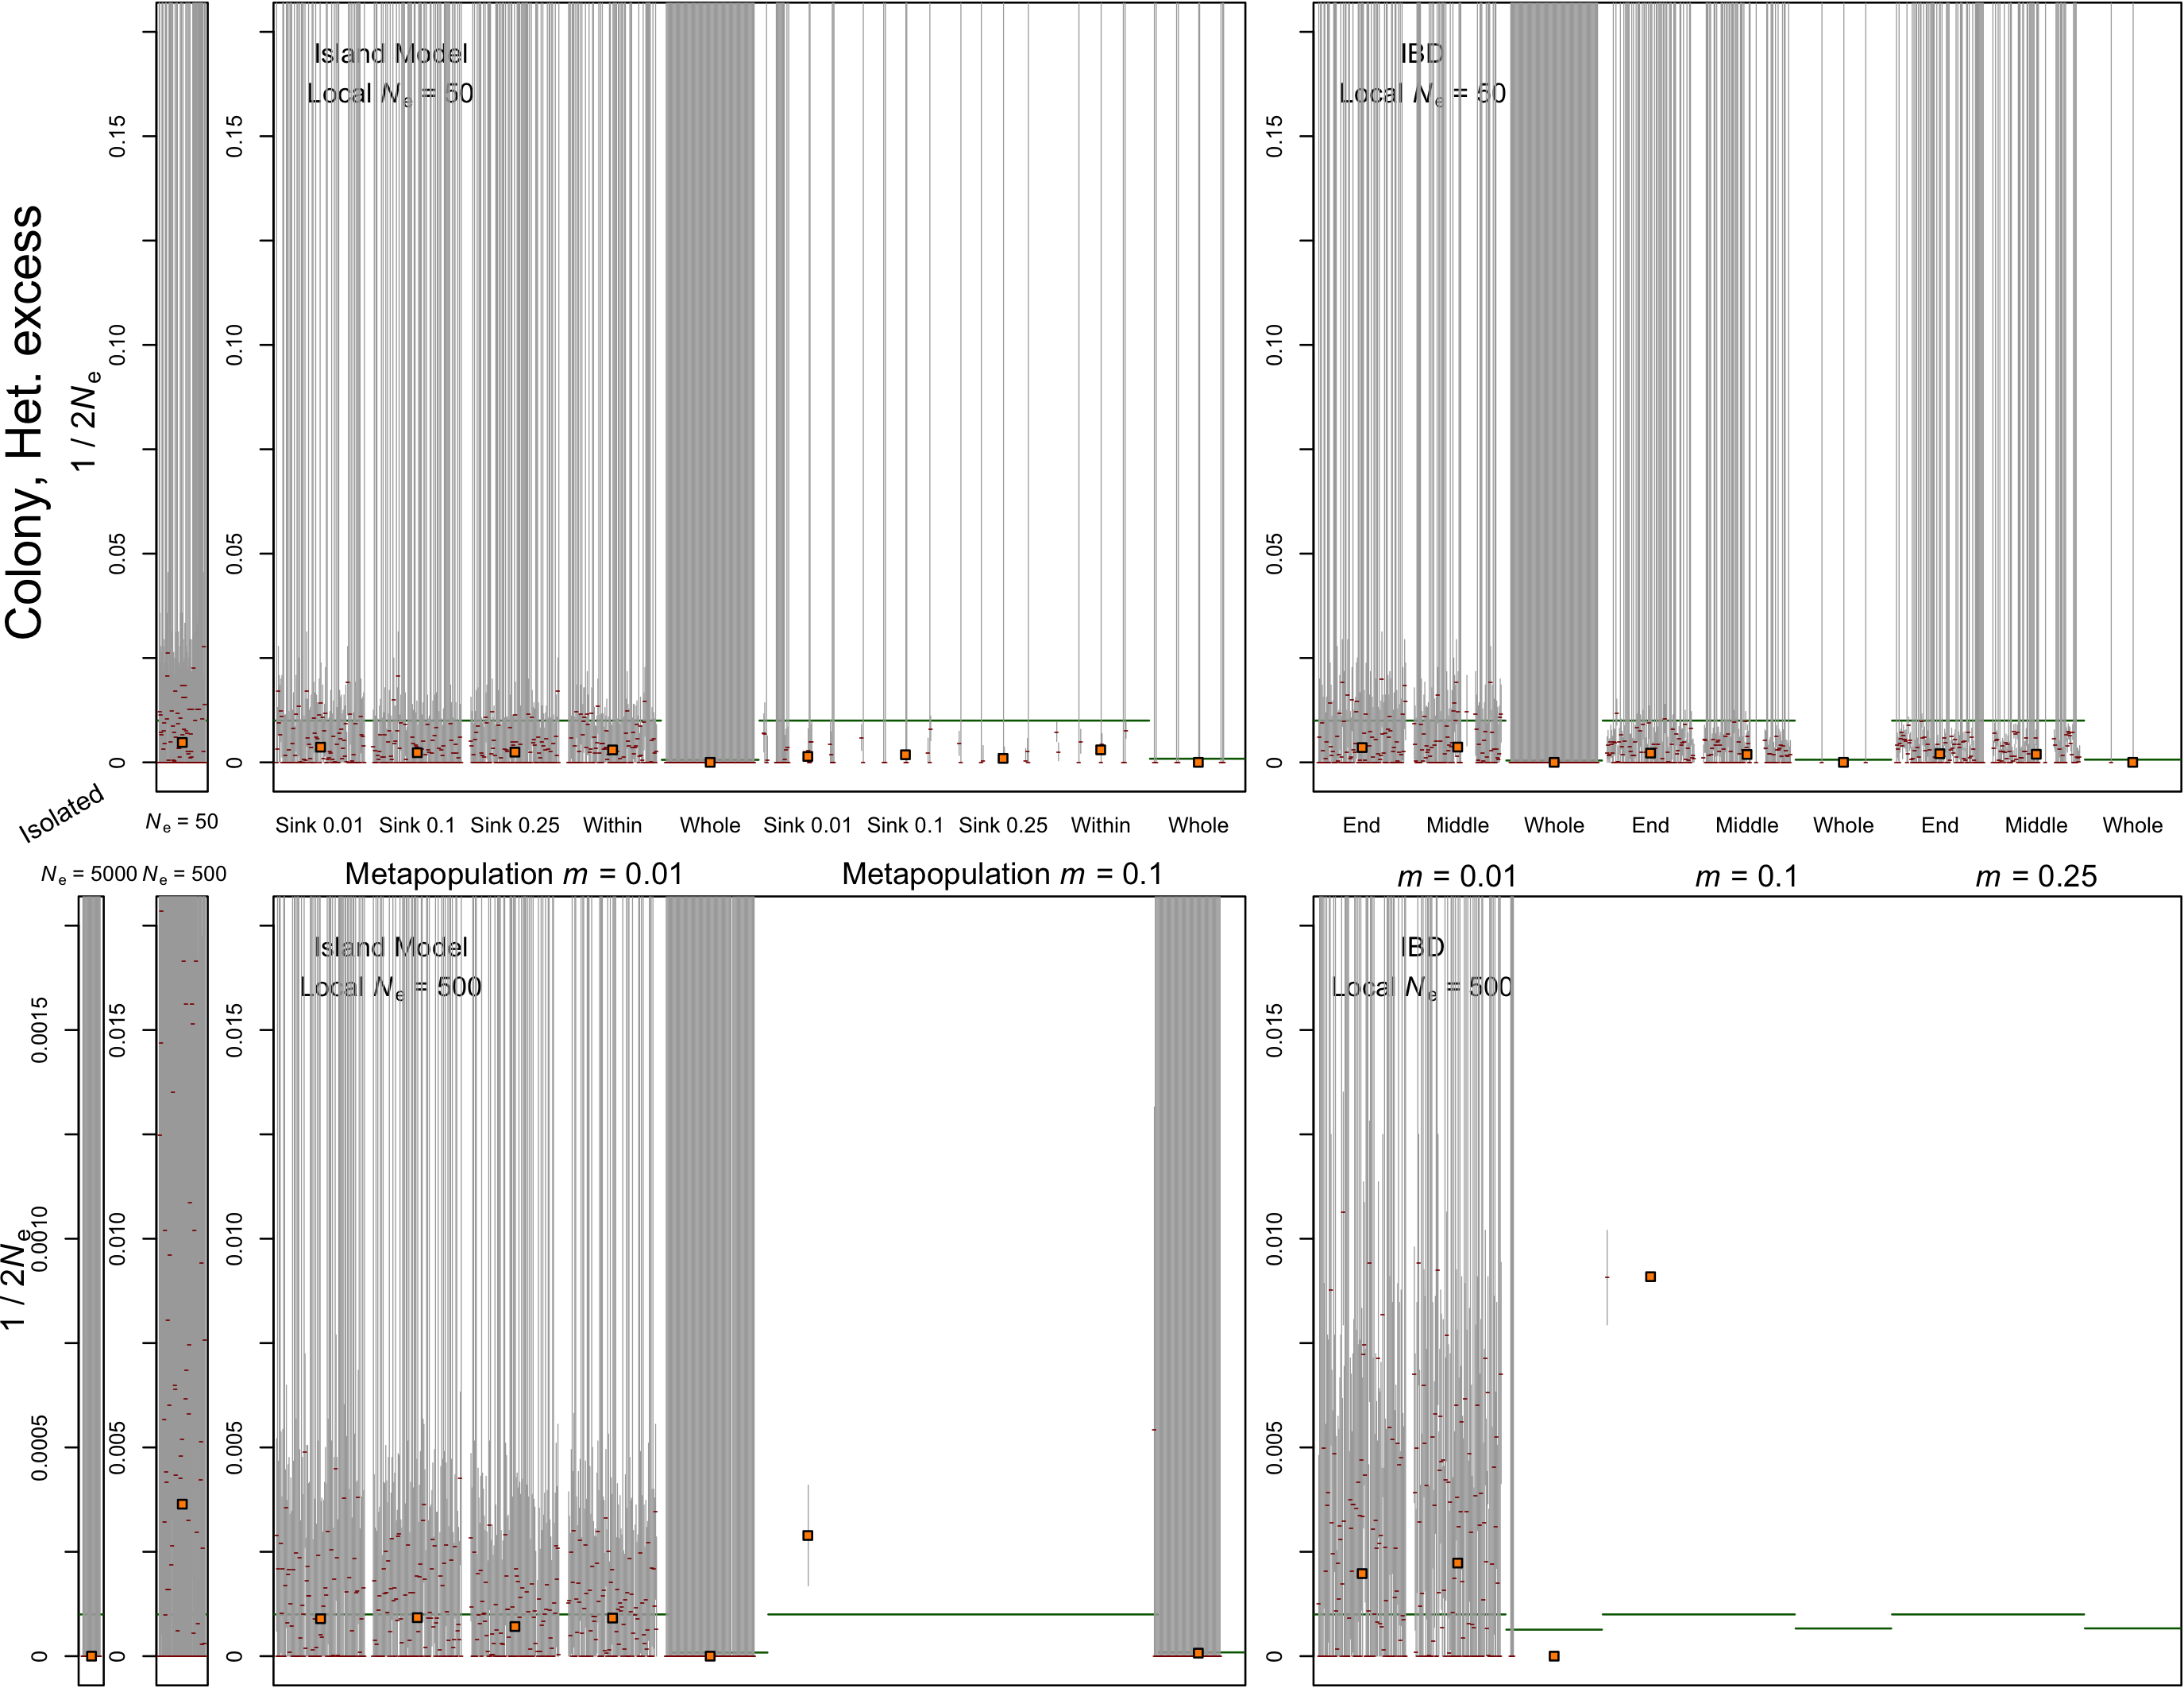
\includegraphics[width=0.8\linewidth]{Figures/SuppFigures/FigureS5a__ColonyHetRawResults.png}}
\caption[All replicate estimated $N_e$ values for \textsc{colony2}'s heterozygote excess method across all scenarios.]{All replicate estimated $N_e$ values for \textsc{colony2}'s heterozygote excess method across all scenarios. True $N_e$ is shown by the horizontal green lines, point estimates in red with their average indicate by the orange square, and $95\%$ confidence intervals by gray vertical lines. $y$-axis is $\frac{1}{2 N_e}$ and scenarios are shown across the $x$-axis, labeled in the center row. The three isolated, no migration cases are shown on the left, followed by the island model migration cases in the middle and the stepping stone IBD cases on the right, with $N_e = 50$ along the top row and 500 along the bottom row. Missing data indicates replicates that were not run due to computational limits (see text).}
\label{fig:supp_colonyhet}
\end{figure}


\begin{figure}[h!]
\centering
\makebox[\textwidth]{
        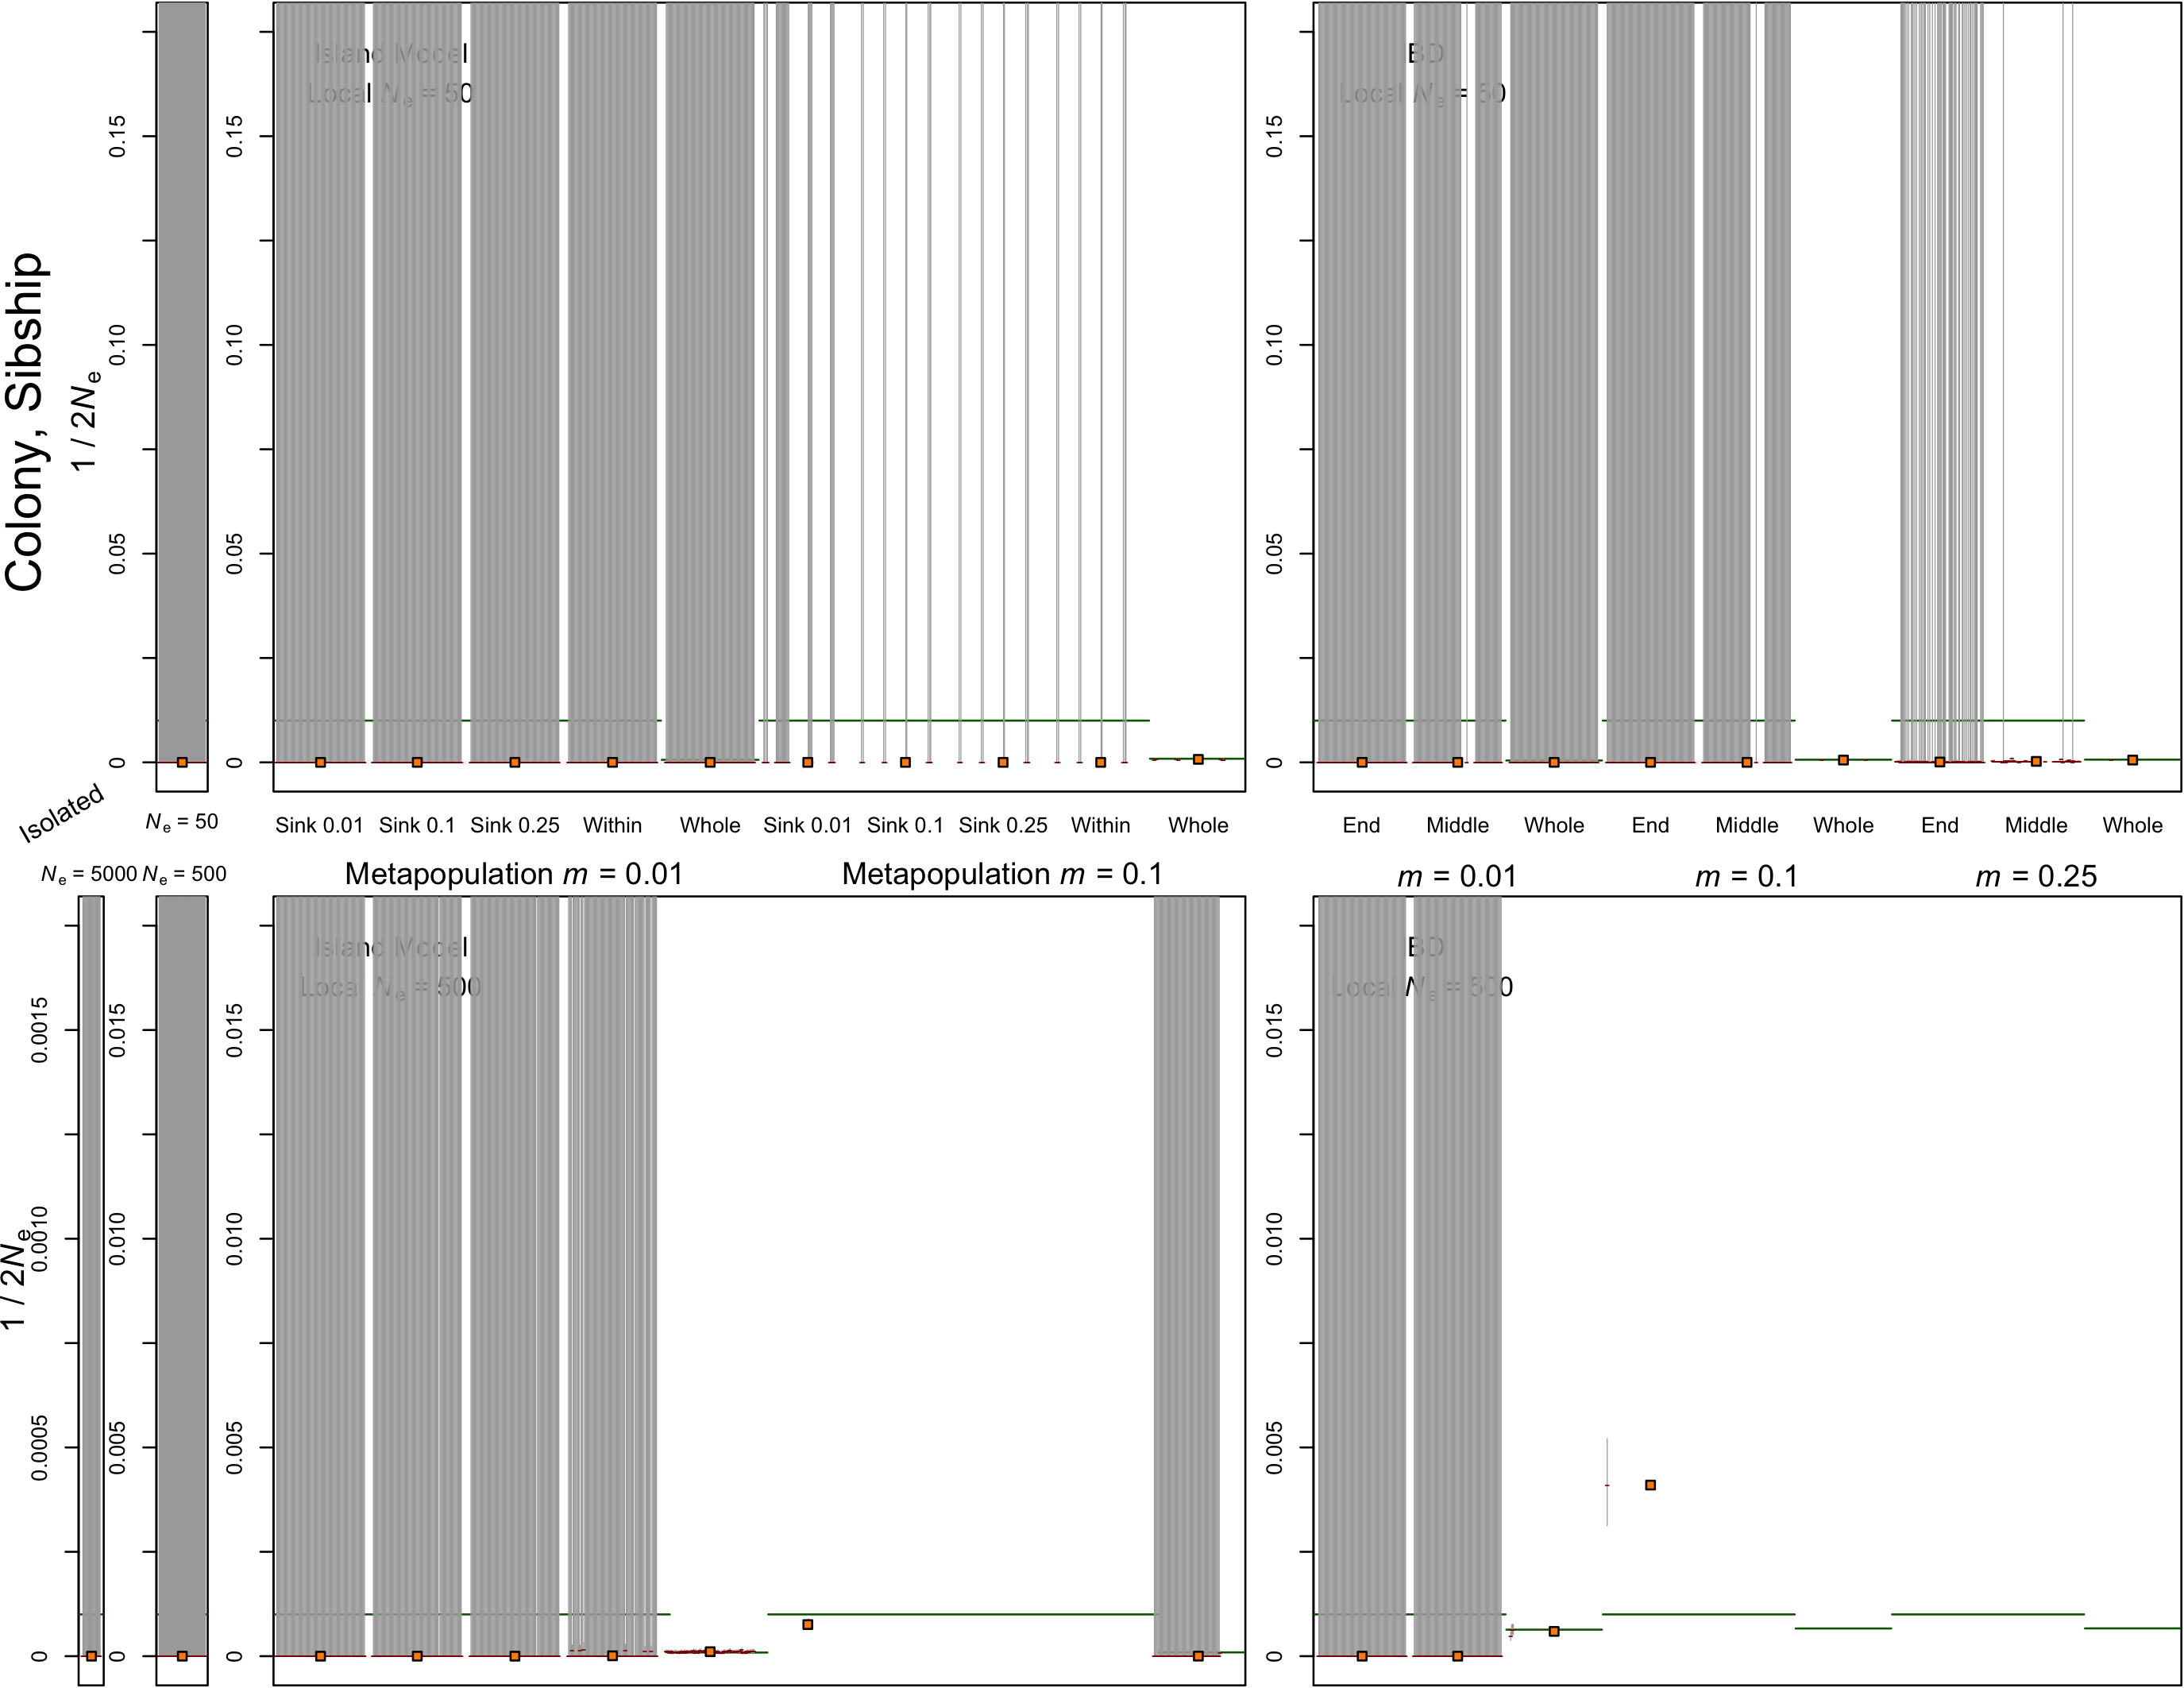
\includegraphics[width=0.8\linewidth]{Figures/SuppFigures/FigureS5b__ColonySibRawResults.png}}
\caption[All replicate estimated $N_e$ values for \textsc{colony2}'s sibship likelihood method across all scenarios.]{All replicate estimated $N_e$ values for \textsc{colony2}'s sibship likelihood method across all scenarios. True $N_e$ is shown by the horizontal green lines, point estimates in red with their average indicate by the orange square, and $95\%$ confidence intervals by gray vertical lines. $y$-axis is $\frac{1}{2 N_e}$ and scenarios are shown across the $x$-axis, labeled in the center row. The three isolated, no migration cases are shown on the left, followed by the island model migration cases in the middle and the stepping stone IBD cases on the right, with $N_e = 50$ along the top row and 500 along the bottom row. Missing data indicates replicates that were not run due to computational limits (see text).}
\label{fig:supp_colonysib}
\end{figure}


\begin{figure}[h!]
\centering
\makebox[\textwidth]{
        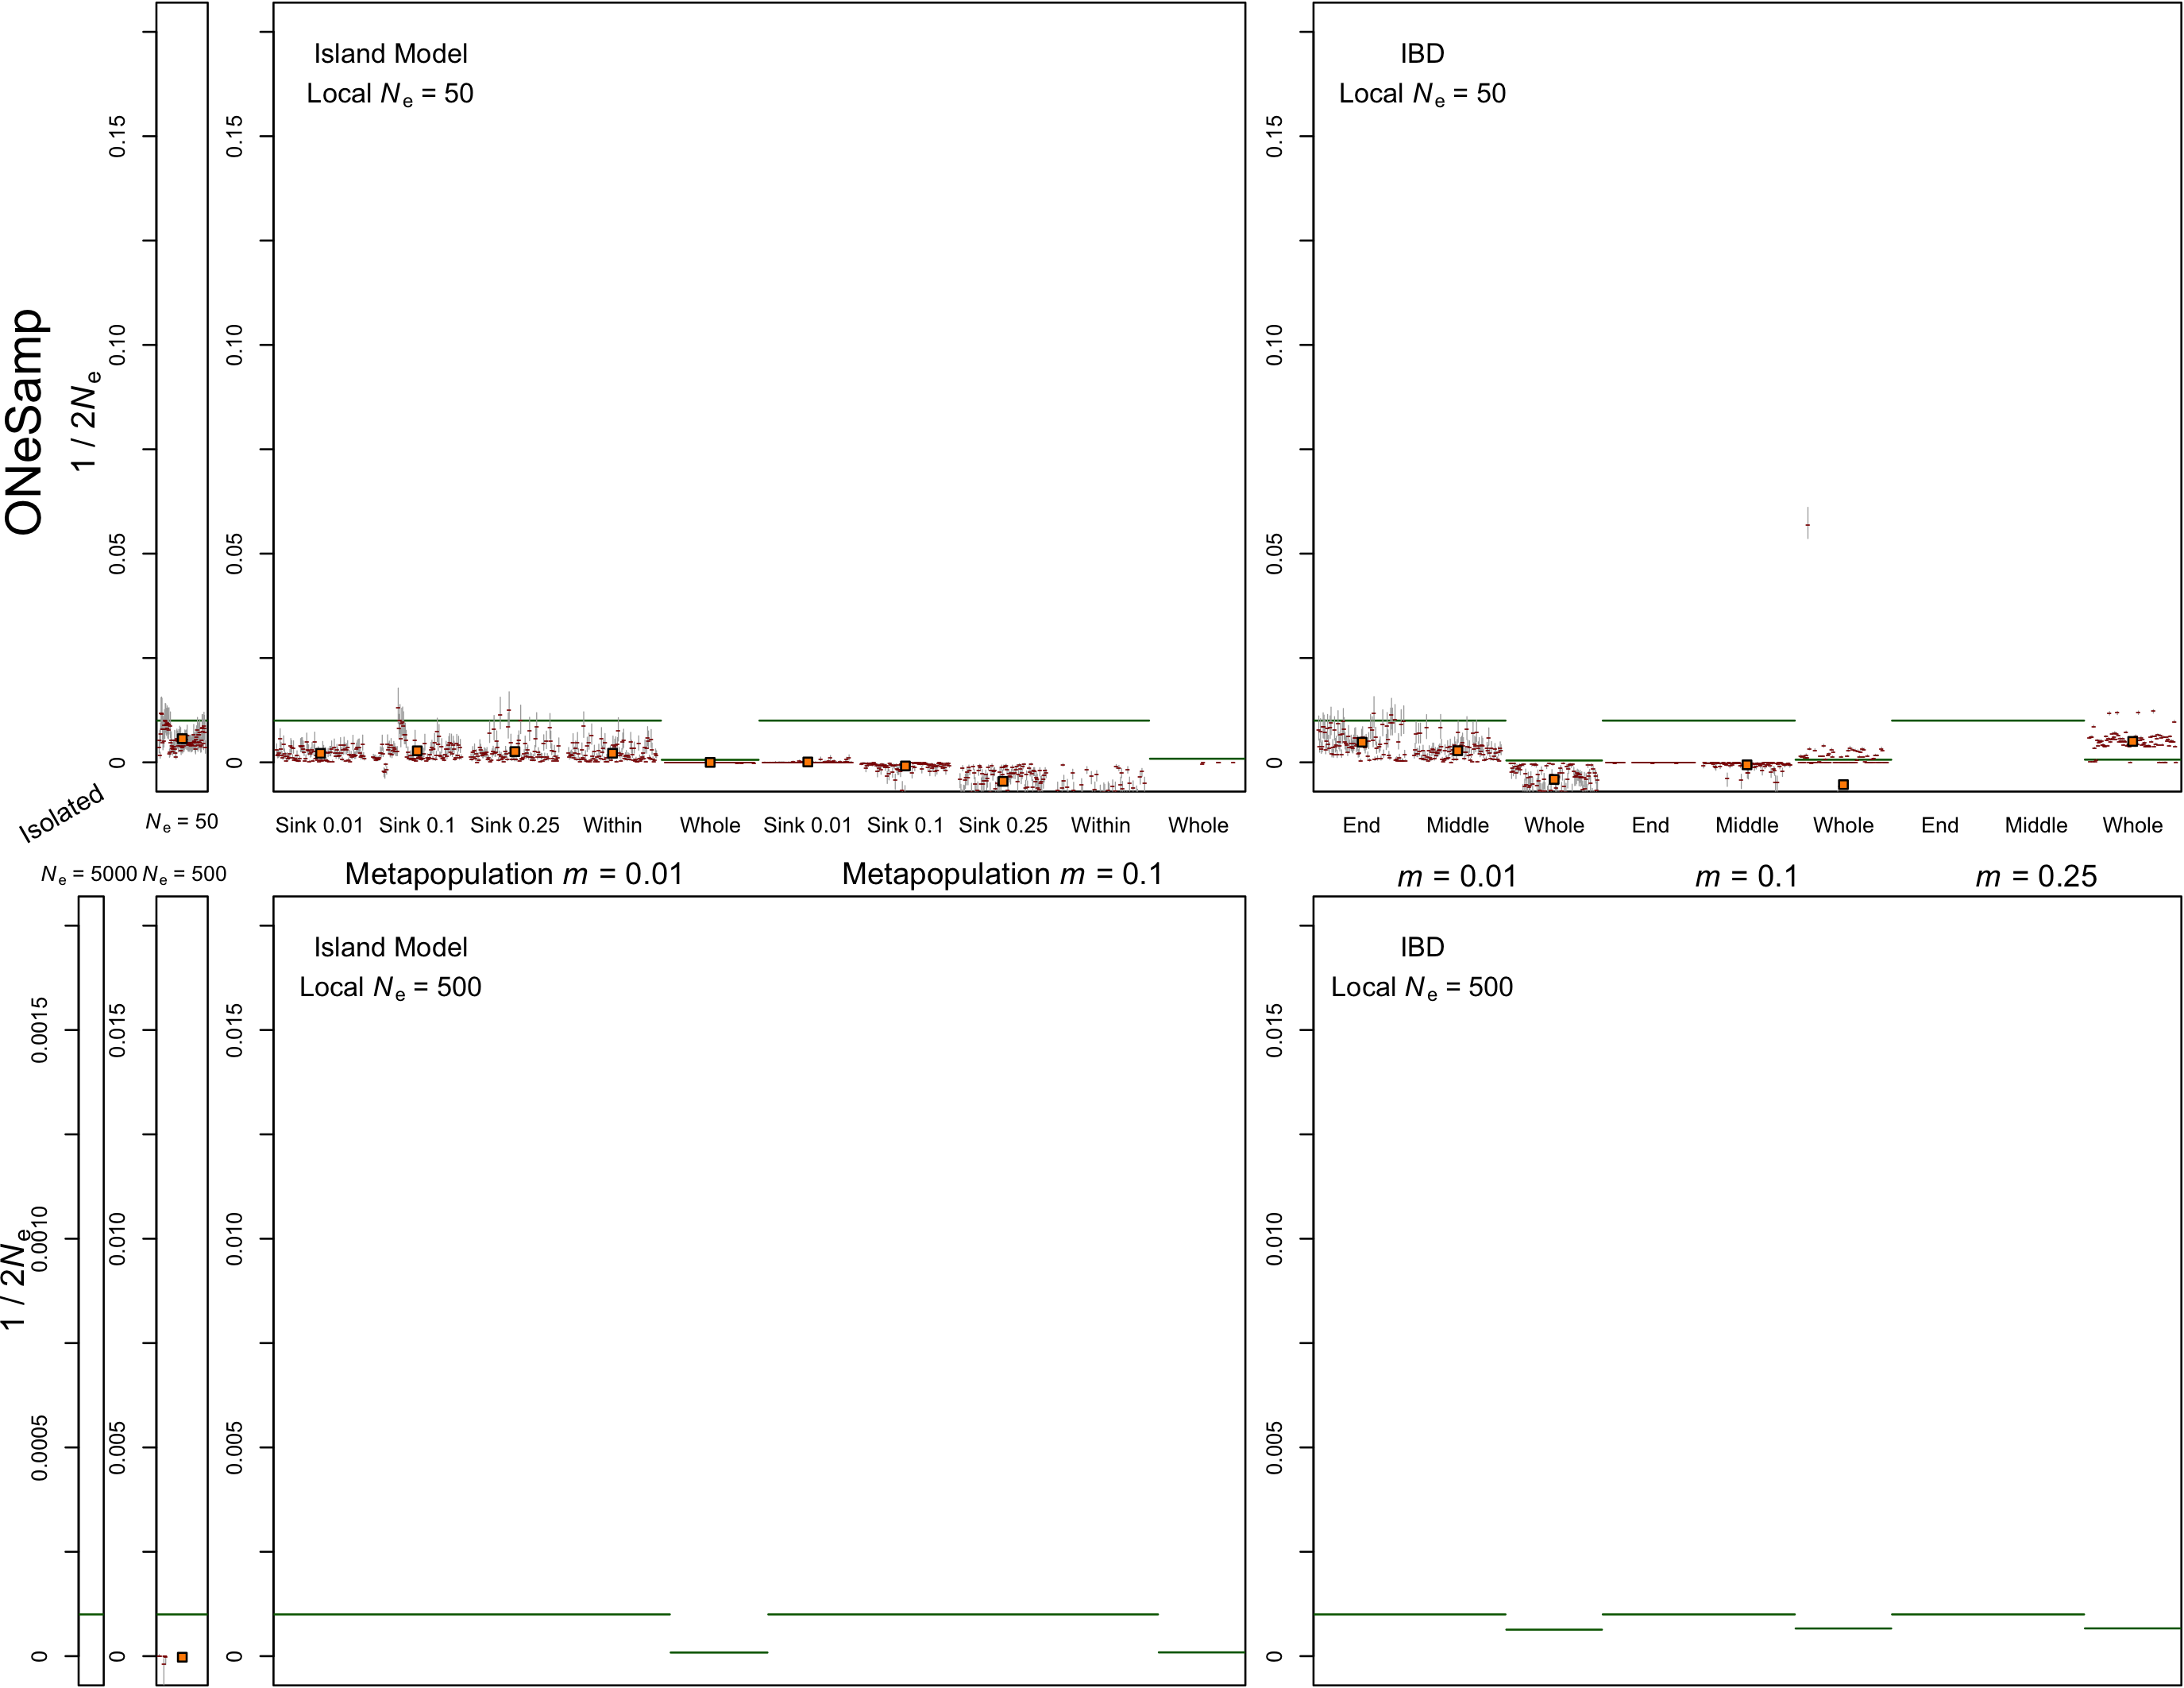
\includegraphics[width=0.8\linewidth]{Figures/SuppFigures/FigureS6__ONeSampRawResults.png}}
\caption[All replicate estimated $N_e$ values for \textsc{onesamp} across all scenarios.]{All replicate estimated $N_e$ values for \textsc{onesamp} across all scenarios. True $N_e$ is shown by the horizontal green lines, point estimates in red with their average indicate by the orange square, and $95\%$ confidence intervals by gray vertical lines. $y$-axis is $\frac{1}{2 N_e}$ and scenarios are shown across the $x$-axis, labeled in the center row. The three isolated, no migration cases are shown on the left, followed by the island model migration cases in the middle and the stepping stone IBD cases on the right, with $N_e = 50$ along the top row and 500 along the bottom row. Missing data (i.e. all 500 and 5,000 patch sizes except a few isolated 500) indicates replicates that were not run due to computational limits (see text).}
\label{fig:supp_onesamp}
\end{figure}


\begin{figure}[h!]
\centering
\makebox[\textwidth]{
        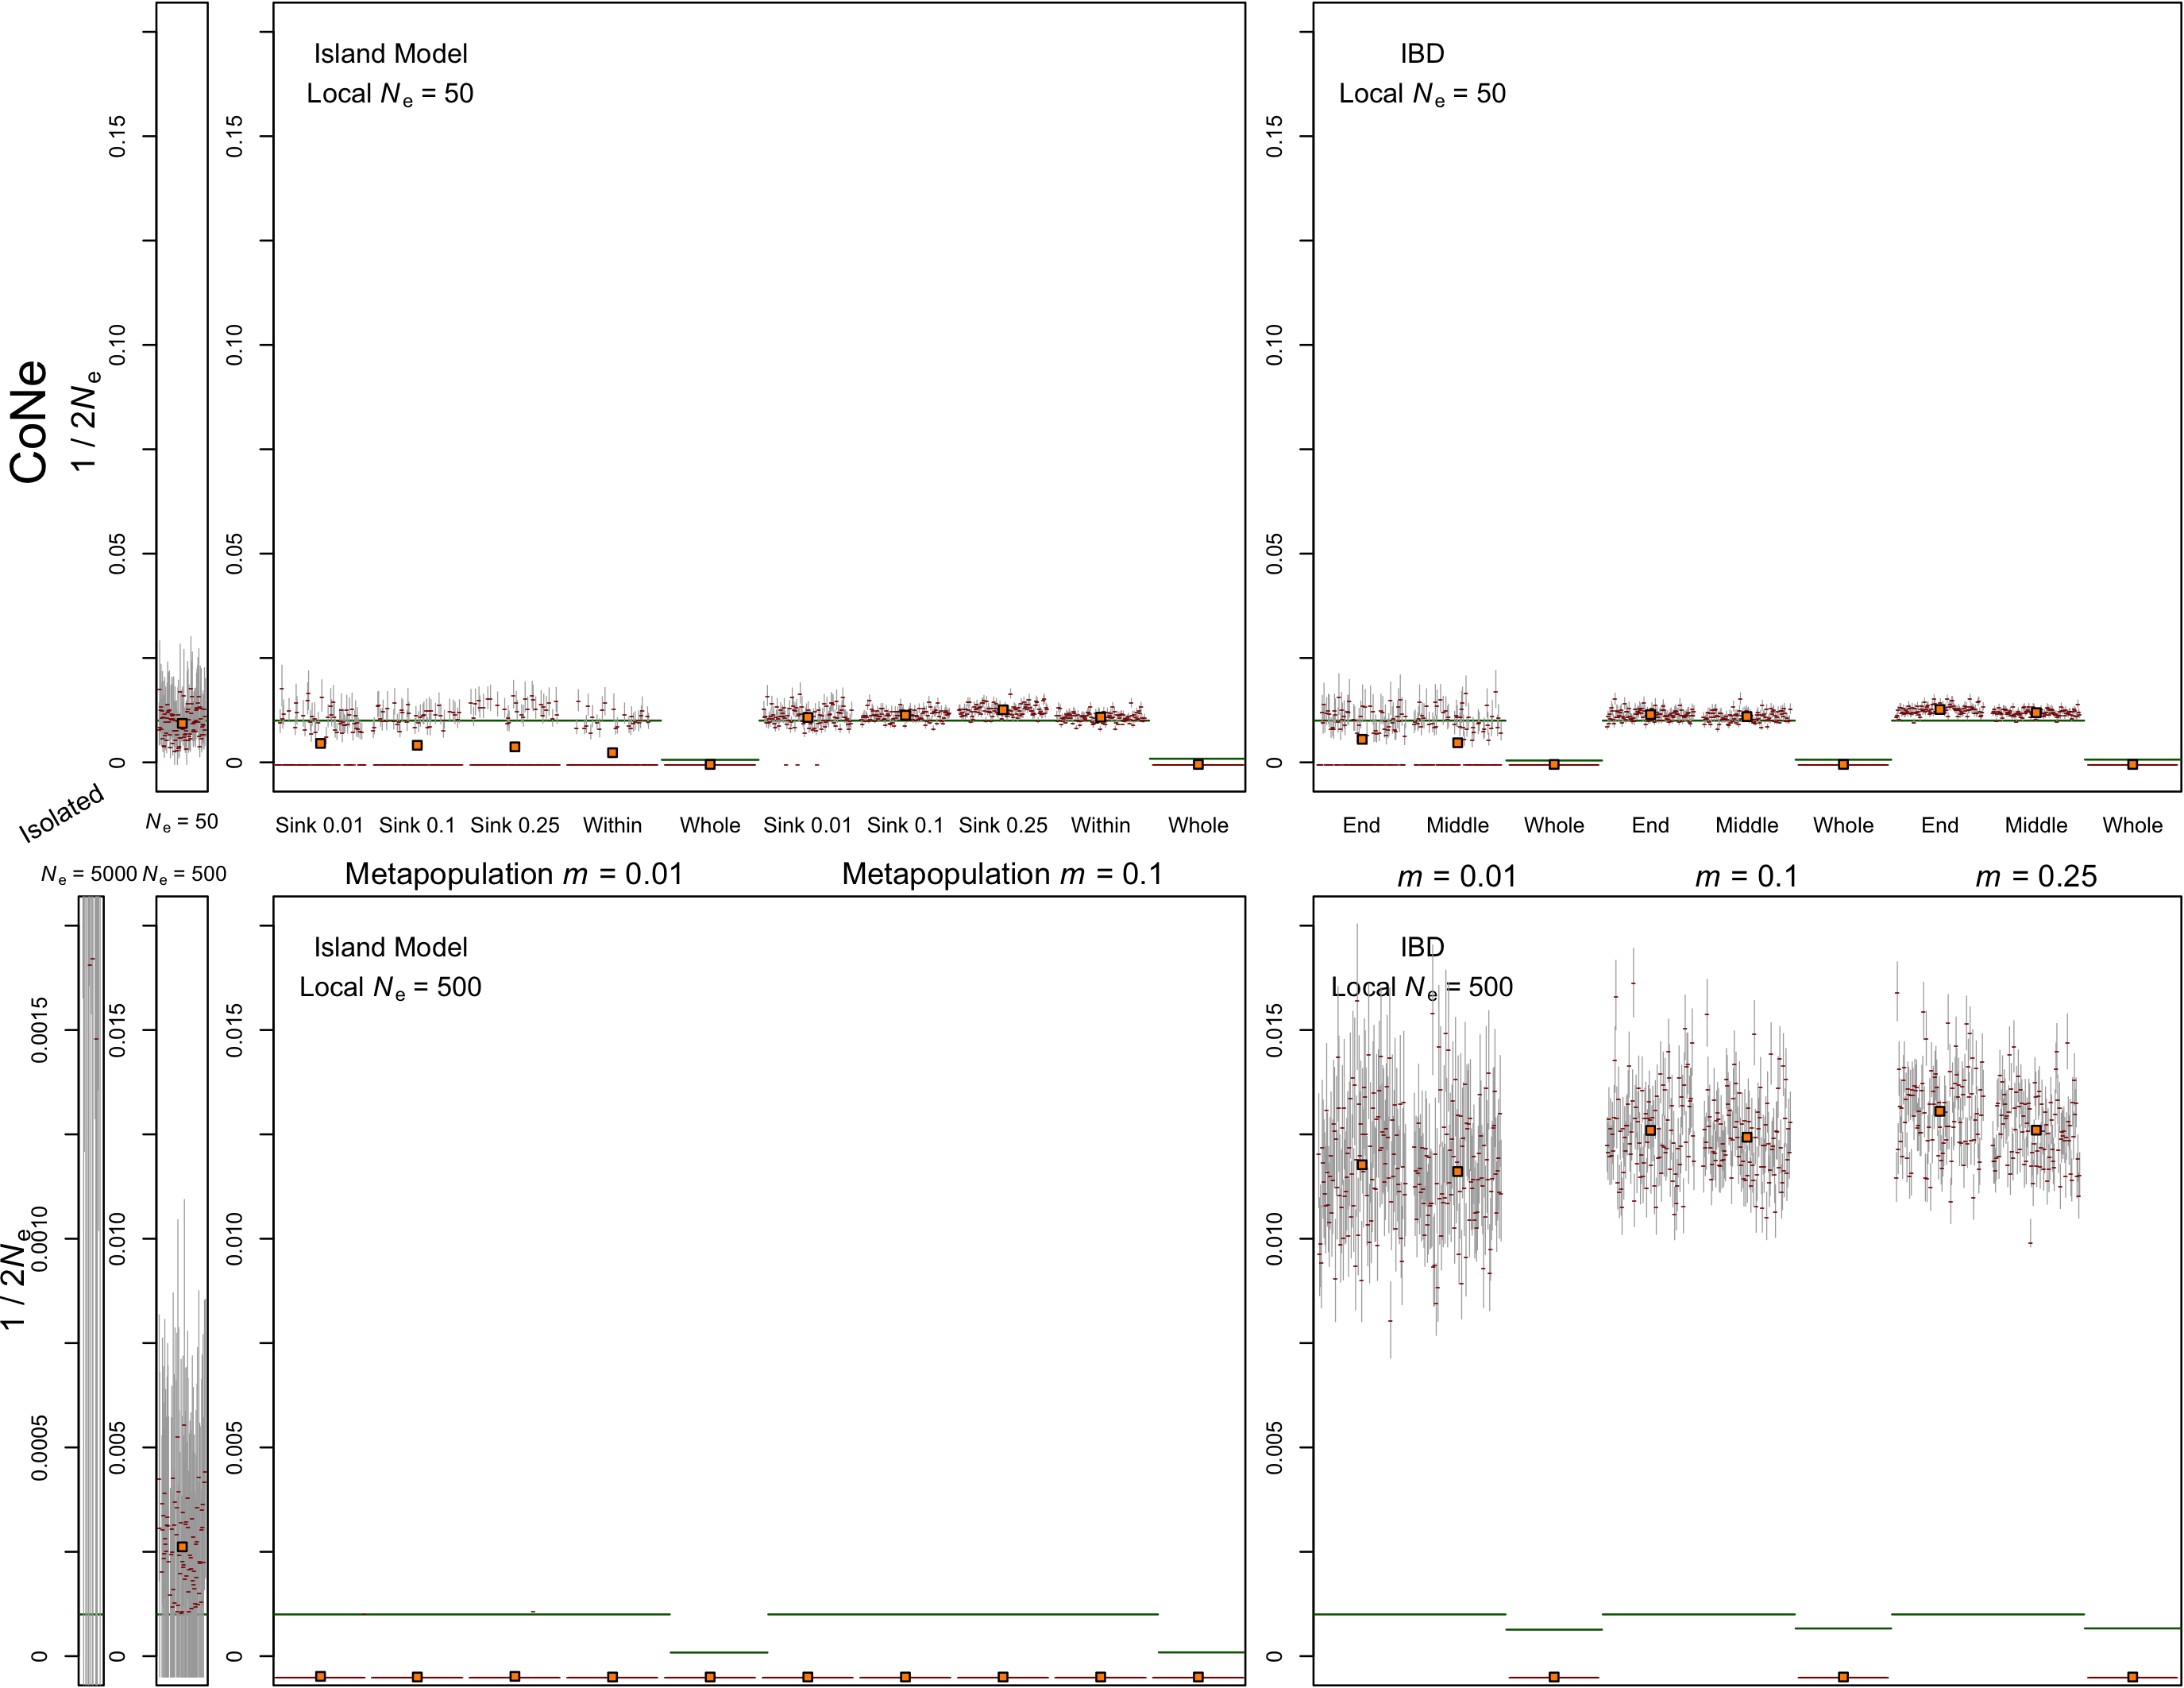
\includegraphics[width=0.8\linewidth]{Figures/SuppFigures/FigureS7__CoNeRawResults.png}}
\caption[All replicate estimated $N_e$ values for \textsc{cone} across all scenarios.]{All replicate estimated $N_e$ values for \textsc{cone} across all scenarios. True $N_e$ is shown by the horizontal green lines, point estimates in red with their average indicate by the orange square, and $95\%$ confidence intervals by gray vertical lines. $y$-axis is $\frac{1}{2 N_e}$ and scenarios are shown across the $x$-axis, labeled in the center row. The three isolated, no migration cases are shown on the left, followed by the island model migration cases in the middle and the stepping stone IBD cases on the right, with $N_e = 50$ along the top row and 500 along the bottom row. Estimates below zero are those for which the program produced values of -999.99, indicating an $N_e$ outside of the specified prior (see text).}
\label{fig:supp_cone}
\end{figure}


\begin{figure}[h!]
\centering
\makebox[\textwidth]{
        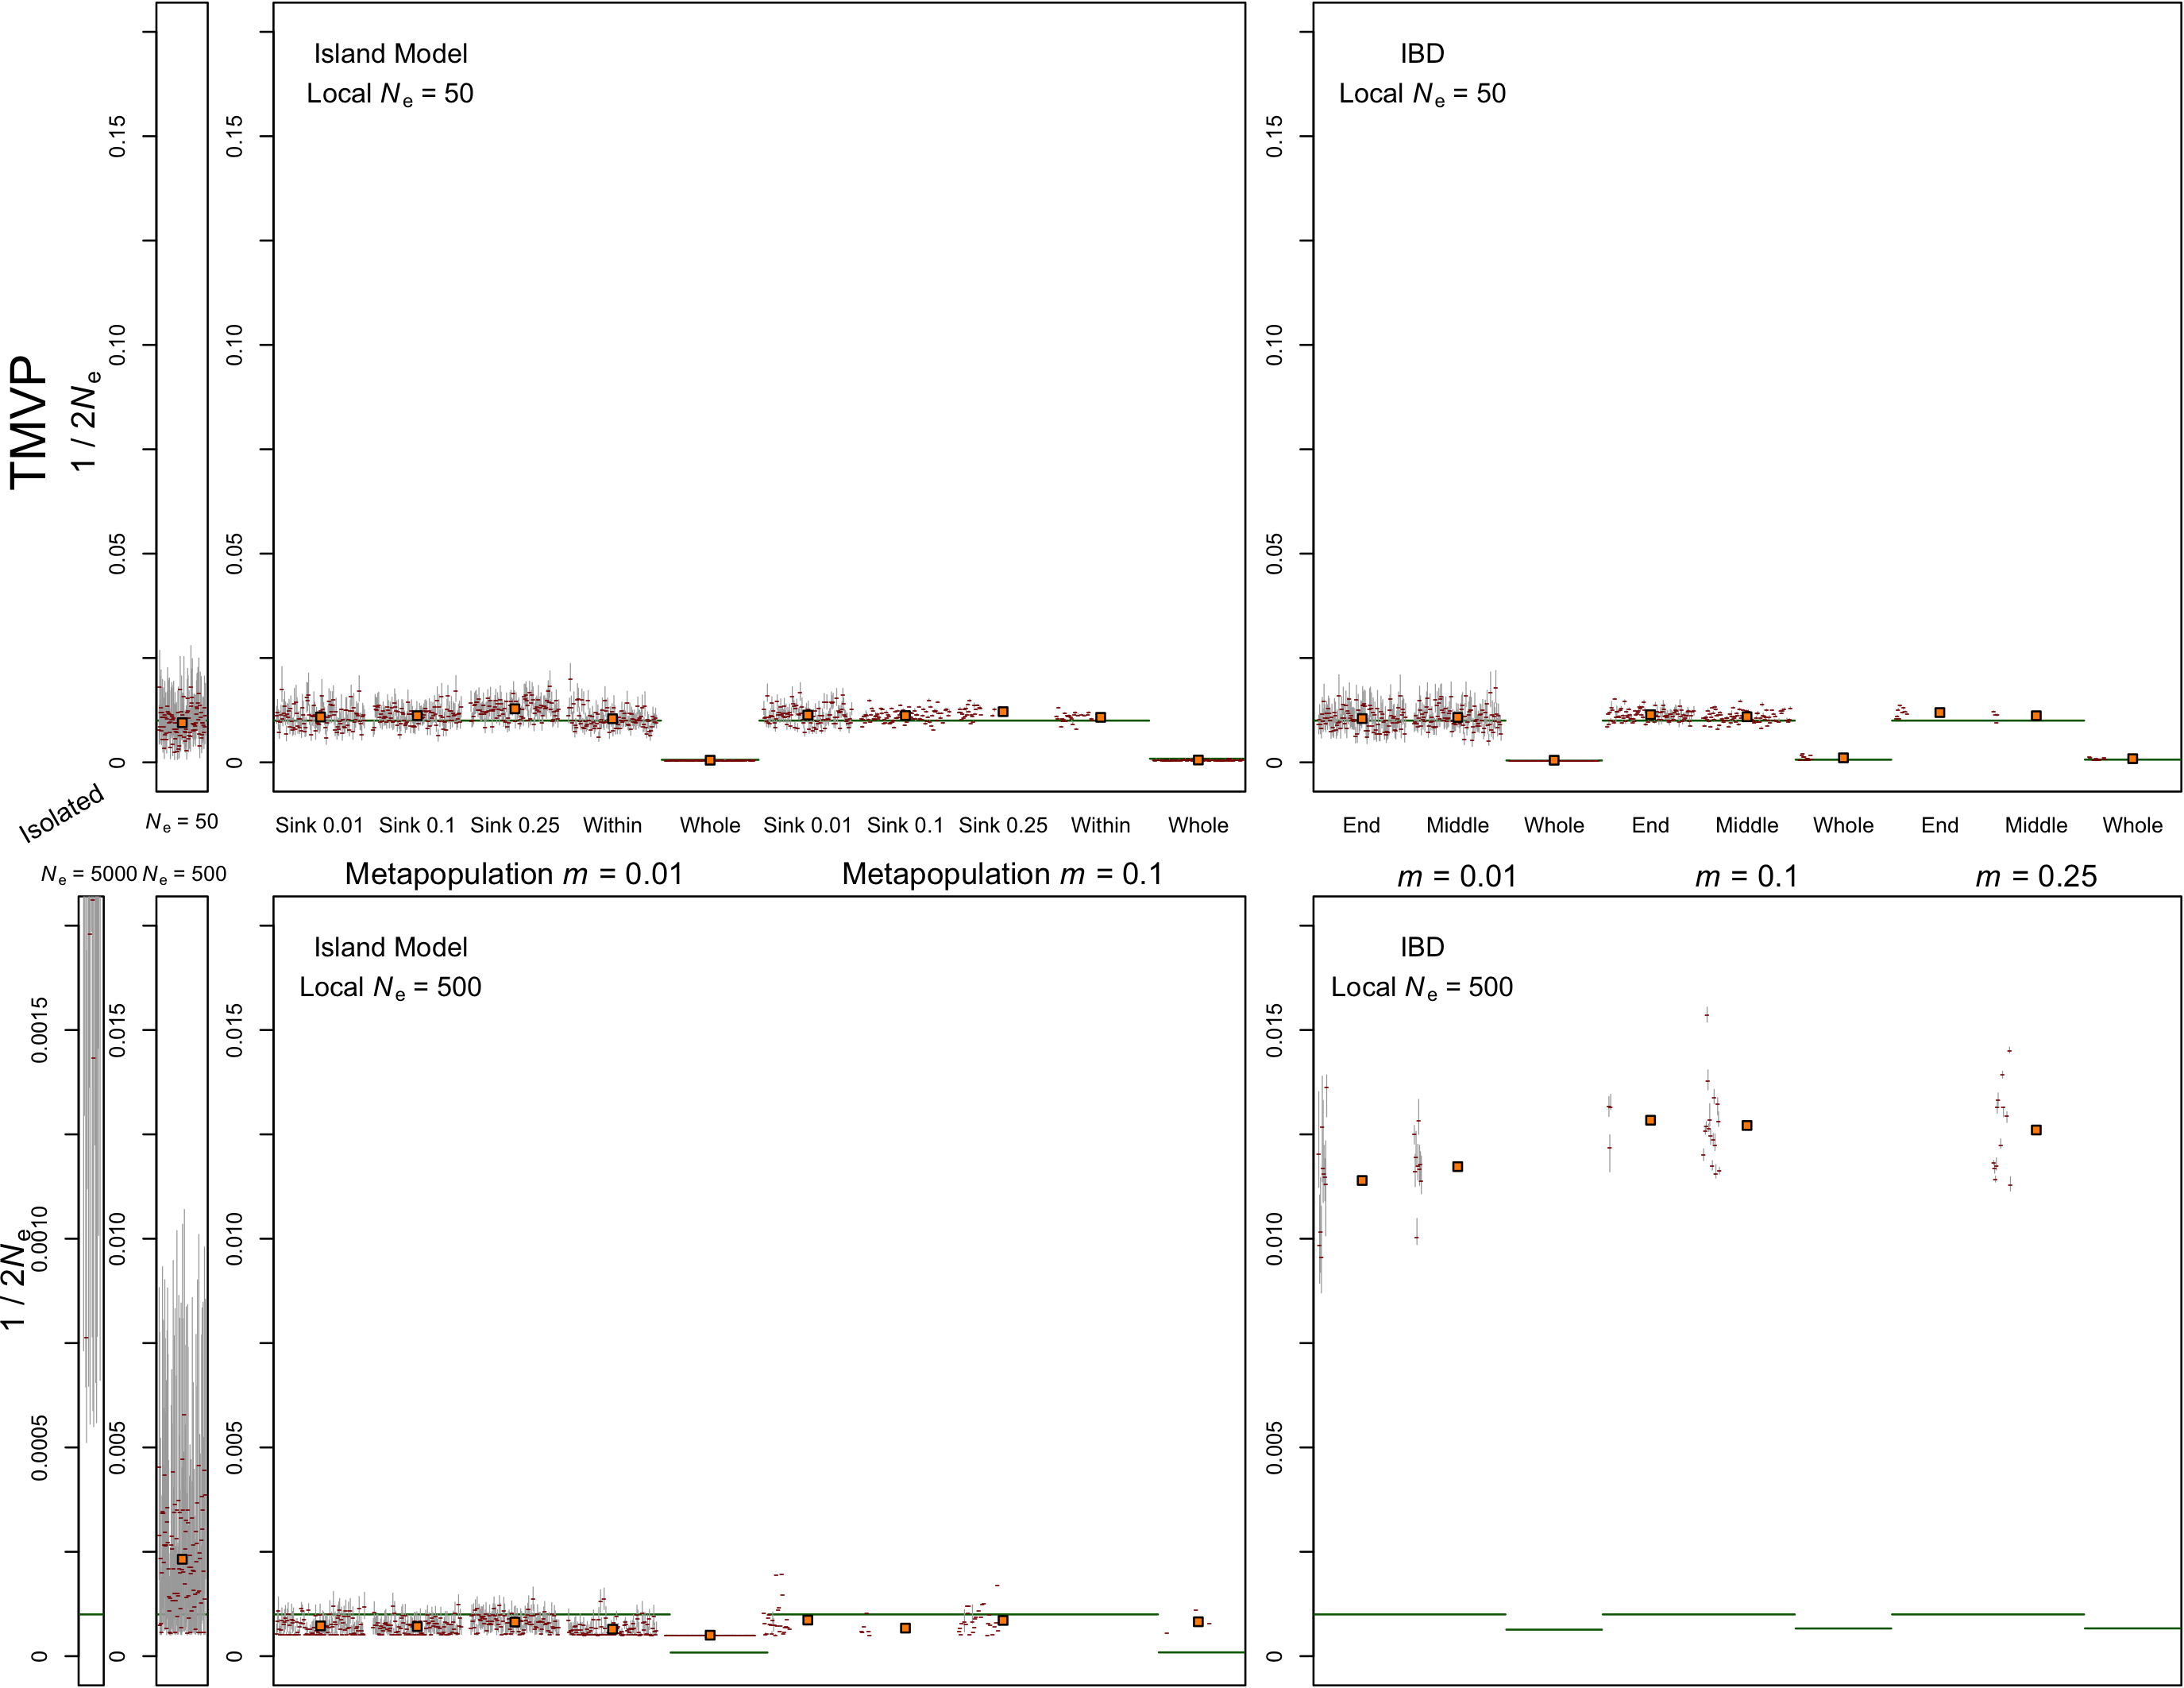
\includegraphics[width=0.8\linewidth]{Figures/SuppFigures/FigureS8__TMVPRawResults.png}}
\caption[All replicate estimated $N_e$ values for \textsc{tmvp} across all scenarios.]{All replicate estimated $N_e$ values for \textsc{tmvp} across all scenarios. True $N_e$ is shown by the horizontal green lines, point estimates in red with their average indicate by the orange square, and $95\%$ confidence intervals by gray vertical lines. $y$-axis is $\frac{1}{2 N_e}$ and scenarios are shown across the $x$-axis, labeled in the center row. The three isolated, no migration cases are shown on the left, followed by the island model migration cases in the middle and the stepping stone IBD cases on the right, with $N_e = 50$ along the top row and 500 along the bottom row. Missing data indicates replicates that were not run due to lack of convergence for reasonable parameter values (see text).}
\label{fig:supp_tmvp}
\end{figure}


\begin{figure}[h!]
\centering
\makebox[\textwidth]{
        \includegraphics[width=0.8\linewidth]{Figures/SuppFigures/.png}}
\caption[All replicate estimated $N_e$ values for \textsc{neestimator}'s heterozygote excess method across all scenarios.]{All replicate estimated $N_e$ values for \textsc{neestimator}'s heterozygote excess method across all scenarios. True $N_e$ is shown by the horizontal green lines, point estimates in red with their average indicate by the orange square, and $95\%$ confidence intervals by gray vertical lines. $y$-axis is $\frac{1}{2 N_e}$ and scenarios are shown across the $x$-axis, labeled in the center row. The three isolated, no migration cases are shown on the left, followed by the island model migration cases in the middle and the stepping stone IBD cases on the right, with $N_e = 50$ along the top row and 500 along the bottom row.}
\label{fig:supp_}
\end{figure}


\begin{figure}[h!]
\centering
\makebox[\textwidth]{
        \includegraphics[width=0.8\linewidth]{Figures/SuppFigures/.png}}
\caption[All replicate estimated $N_e$ values for \textsc{neestimator}'s coancestry method across all scenarios.]{All replicate estimated $N_e$ values for \textsc{neestimator}'s coancestry method across all scenarios. True $N_e$ is shown by the horizontal green lines, point estimates in red with their average indicate by the orange square, and $95\%$ confidence intervals by gray vertical lines. $y$-axis is $\frac{1}{2 N_e}$ and scenarios are shown across the $x$-axis, labeled in the center row. The three isolated, no migration cases are shown on the left, followed by the island model migration cases in the middle and the stepping stone IBD cases on the right, with $N_e = 50$ along the top row and 500 along the bottom row.}
\label{fig:supp_}
\end{figure}


\begin{figure}[h!]
\centering
\makebox[\textwidth]{
        \includegraphics[width=0.8\linewidth]{Figures/SuppFigures/.png}}
\caption[All replicate estimated $N_e$ values for \textsc{neestimator}'s Pollak method across all scenarios.]{All replicate estimated $N_e$ values for \textsc{neestimator}'s Pollak method across all scenarios. True $N_e$ is shown by the horizontal green lines, point estimates in red with their average indicate by the orange square, and $95\%$ confidence intervals by gray vertical lines. $y$-axis is $\frac{1}{2 N_e}$ and scenarios are shown across the $x$-axis, labeled in the center row. The three isolated, no migration cases are shown on the left, followed by the island model migration cases in the middle and the stepping stone IBD cases on the right, with $N_e = 50$ along the top row and 500 along the bottom row. Negative estimates are shown, but in analyses were changed to infinite $N_e$ as indicated by the method's authors (see text).}
\label{fig:supp_}
\end{figure}


\begin{figure}[h!]
\centering
\makebox[\textwidth]{
        \includegraphics[width=0.8\linewidth]{Figures/SuppFigures/.png}}
\caption[All replicate estimated $N_e$ values for \textsc{neestimator}'s Nei and Tajima method across all scenarios.]{All replicate estimated $N_e$ values for \textsc{neestimator}'s Nei and Tajima method across all scenarios. True $N_e$ is shown by the horizontal green lines, point estimates in red with their average indicate by the orange square, and $95\%$ confidence intervals by gray vertical lines. $y$-axis is $\frac{1}{2 N_e}$ and scenarios are shown across the $x$-axis, labeled in the center row. The three isolated, no migration cases are shown on the left, followed by the island model migration cases in the middle and the stepping stone IBD cases on the right, with $N_e = 50$ along the top row and 500 along the bottom row. Negative estimates are shown, but in analyses were changed to infinite $N_e$ as indicated by the method's authors (see text).}
\label{fig:supp_}
\end{figure}


\begin{figure}[h!]
\centering
\makebox[\textwidth]{
        \includegraphics[width=0.8\linewidth]{Figures/SuppFigures/.png}}
\caption[All replicate estimated $N_e$ values for \textsc{neestimator}'s Jorde and Ryman method across all scenarios.]{All replicate estimated $N_e$ values for \textsc{neestimator}'s Jorde and Ryman method across all scenarios. True $N_e$ is shown by the horizontal green lines, point estimates in red with their average indicate by the orange square, and $95\%$ confidence intervals by gray vertical lines. $y$-axis is $\frac{1}{2 N_e}$ and scenarios are shown across the $x$-axis, labeled in the center row. The three isolated, no migration cases are shown on the left, followed by the island model migration cases in the middle and the stepping stone IBD cases on the right, with $N_e = 50$ along the top row and 500 along the bottom row. Negative estimates are shown, but in analyses were changed to infinite $N_e$ as indicated by the method's authors (see text).}
\label{fig:supp_}
\end{figure}


\begin{figure}[h!]
\centering
\makebox[\textwidth]{
        \includegraphics[width=0.8\linewidth]{Figures/SuppFigures/.png}}
\caption[All replicate estimated $N_e$ values for the average of \textsc{mlne}'s likelihood and moment methods across all scenarios.]{All replicate estimated $N_e$ values for the average of \textsc{mlne}'s likelihood and moment methods across all scenarios. True $N_e$ is shown by the horizontal green lines, point estimates in red with their average indicate by the orange square. $y$-axis is $\frac{1}{2 N_e}$ and scenarios are shown across the $x$-axis, labeled in the center row. The three isolated, no migration cases are shown on the left, followed by the island model migration cases in the middle and the stepping stone IBD cases on the right, with $N_e = 50$ along the top row and 500 along the bottom row. No confidence intervals are estimated.}
\label{fig:supp_avg1}
\end{figure}


\begin{figure}[h!]
\centering
\makebox[\textwidth]{
        \includegraphics[width=0.8\linewidth]{Figures/SuppFigures/.png}}
\caption[All replicate estimated $N_e$ values for the average of \textsc{neestimator}'s \textsc{ldne} at both temporal sampling points across all scenarios.]{All replicate estimated $N_e$ values for the average of \textsc{neestimator}'s \textsc{ldne} at both temporal sampling points across all scenarios. True $N_e$ is shown by the horizontal green lines, point estimates in red with their average indicate by the orange square. $y$-axis is $\frac{1}{2 N_e}$ and scenarios are shown across the $x$-axis, labeled in the center row. The three isolated, no migration cases are shown on the left, followed by the island model migration cases in the middle and the stepping stone IBD cases on the right, with $N_e = 50$ along the top row and 500 along the bottom row. No confidence intervals are estimated.}
\label{fig:supp_avg2}
\end{figure}


\begin{figure}[h!]
\centering
\makebox[\textwidth]{
        \includegraphics[width=0.8\linewidth]{Figures/SuppFigures/.png}}
\caption[All replicate estimated $N_e$ values for the average of \textsc{mlne}'s likelihood and moment methods with \textsc{neestimator}'s \textsc{ldne} estimates at both temporal samples across all scenarios.]{All replicate estimated $N_e$ values for the average of \textsc{mlne}'s likelihood and moment methods with \textsc{neestimator}'s \textsc{ldne} estimates at both temporal samples across all scenarios. True $N_e$ is shown by the horizontal green lines, point estimates in red with their average indicate by the orange square. $y$-axis is $\frac{1}{2 N_e}$ and scenarios are shown across the $x$-axis, labeled in the center row. The three isolated, no migration cases are shown on the left, followed by the island model migration cases in the middle and the stepping stone IBD cases on the right, with $N_e = 50$ along the top row and 500 along the bottom row. No confidence intervals are estimated.}
\label{fig:supp_avg3}
\end{figure}


\begin{figure}[h!]
\centering
\makebox[\textwidth]{
        \includegraphics[width=0.8\linewidth]{Figures/SuppFigures/.png}}
\caption[All replicate estimated $N_e$ values for the average of \textsc{mlne}'s likelihood and moment methods with \textsc{tmvp} across all scenarios.]{All replicate estimated $N_e$ values for the average of \textsc{mlne}'s likelihood and moment methods with \textsc{tmvp} across all scenarios. True $N_e$ is shown by the horizontal green lines, point estimates in red with their average indicate by the orange square. Scenarios are shown across the $x$-axis, labeled in the center row. The three isolated, no migration cases are shown on the left, followed by the island model migration cases in the middle and the stepping stone IBD cases on the right, with $N_e = 50$ along the top row and 500 along the bottom row. No confidence intervals are estimated. Missing values are due to lack of \textsc{tmvp} estimates.}
\label{fig:supp_avg4}
\end{figure}


\begin{figure}[h!]
\centering
\makebox[\textwidth]{
        \includegraphics[width=0.8\linewidth]{Figures/SuppFigures/.png}}
\caption[All replicate estimated $N_e$ values for the average of \textsc{mlne}'s likelihood and moment methods with \textsc{neestimator}'s \textsc{ldne} estimates at both temporal samples and \textsc{tmvp} across all scenarios.]{All replicate estimated $N_e$ values for the average of \textsc{mlne}'s likelihood and moment methods with \textsc{neestimator}'s \textsc{ldne} estimates at both temporal samples and \textsc{tmvp} across all scenarios. True $N_e$ is shown by the horizontal green lines, point estimates in red with their average indicate by the orange square. Scenarios are shown across the $x$-axis, labeled in the center row. The three isolated, no migration cases are shown on the left, followed by the island model migration cases in the middle and the stepping stone IBD cases on the right, with $N_e = 50$ along the top row and 500 along the bottom row. No confidence intervals are estimated. Missing values are due to lack of \textsc{tmvp} estimates.}
\label{fig:supp_avg5}
\end{figure}



\end{landscape}






\begin{figure}[h!]
\centering
\makebox[\textwidth]{
        \includegraphics[width=0.8\linewidth]{Figures/SuppFigures/.png}}
\caption[RMSE compared across sample sizes.]{RMSE compared across our standard sample size of 250 (filled points) versus a smaller sample size of 50 individuals (open points). \textsc{ldne} (blue) and \textsc{mlne} likelihood (red) and moment (dark red) methods are compared across isolated populations at $N_e = 50$ and 500, and three migration scenarios each at $N_e = 50$ and 500. The three migration scenarios are shown in order from left to right for each method: the island model demography within metapopulation sampling scenario at $m = 0.01$, sink receiving immigrants at $m = 0.1$ from metapopulation at migration rate $m = 0.1$, and within metapopulation $m = 0.1$, respectively. One result for \textsc{ldne} at $N_e = 500$ showed a reduced RMSE for a population sampled within the metapopulation due to fewer infinite $N_e$ estimates and increased precision around a more biased $N_e$ estimate that nevertheless improved RMSE. Each point represents the average performance for a method over 100 replicate simulations.}
\label{fig:supp_rmsesamp}
\end{figure}


\begin{figure}[h!]
\centering
\makebox[\textwidth]{
        \includegraphics[width=0.8\linewidth]{Figures/SuppFigures/FigureS19__MigSrc-LikMomMethod_combined.png}}
\caption[RMSE of $N_e$ across migration scenarios.]{RMSE of $N_e$ across migration scenarios for \textsc{mlne}'s likelihood (solid lines) and moment (dashed lines) methods when identifying a source population that is the correct source, a related source, an unrelated source, or (see figure S1) the metapopulation as the source. $N_e = 50$ is shown across the top row and $N_e = 500$ across the bottom row. Island model scenarios are in the left panels and stepping stone (IBD) scenarios are in the right panels. Note that a migration source cannot be provided when the whole metapopulation is sampled as one, so these cases are only single populations experiencing migration either as a sink from the metapopulation or a population within the island model or stepping stone metapopulations.}
\label{fig:supp_rmsemig}
\end{figure}


\begin{figure}[h!]
\centering
\makebox[\textwidth]{
        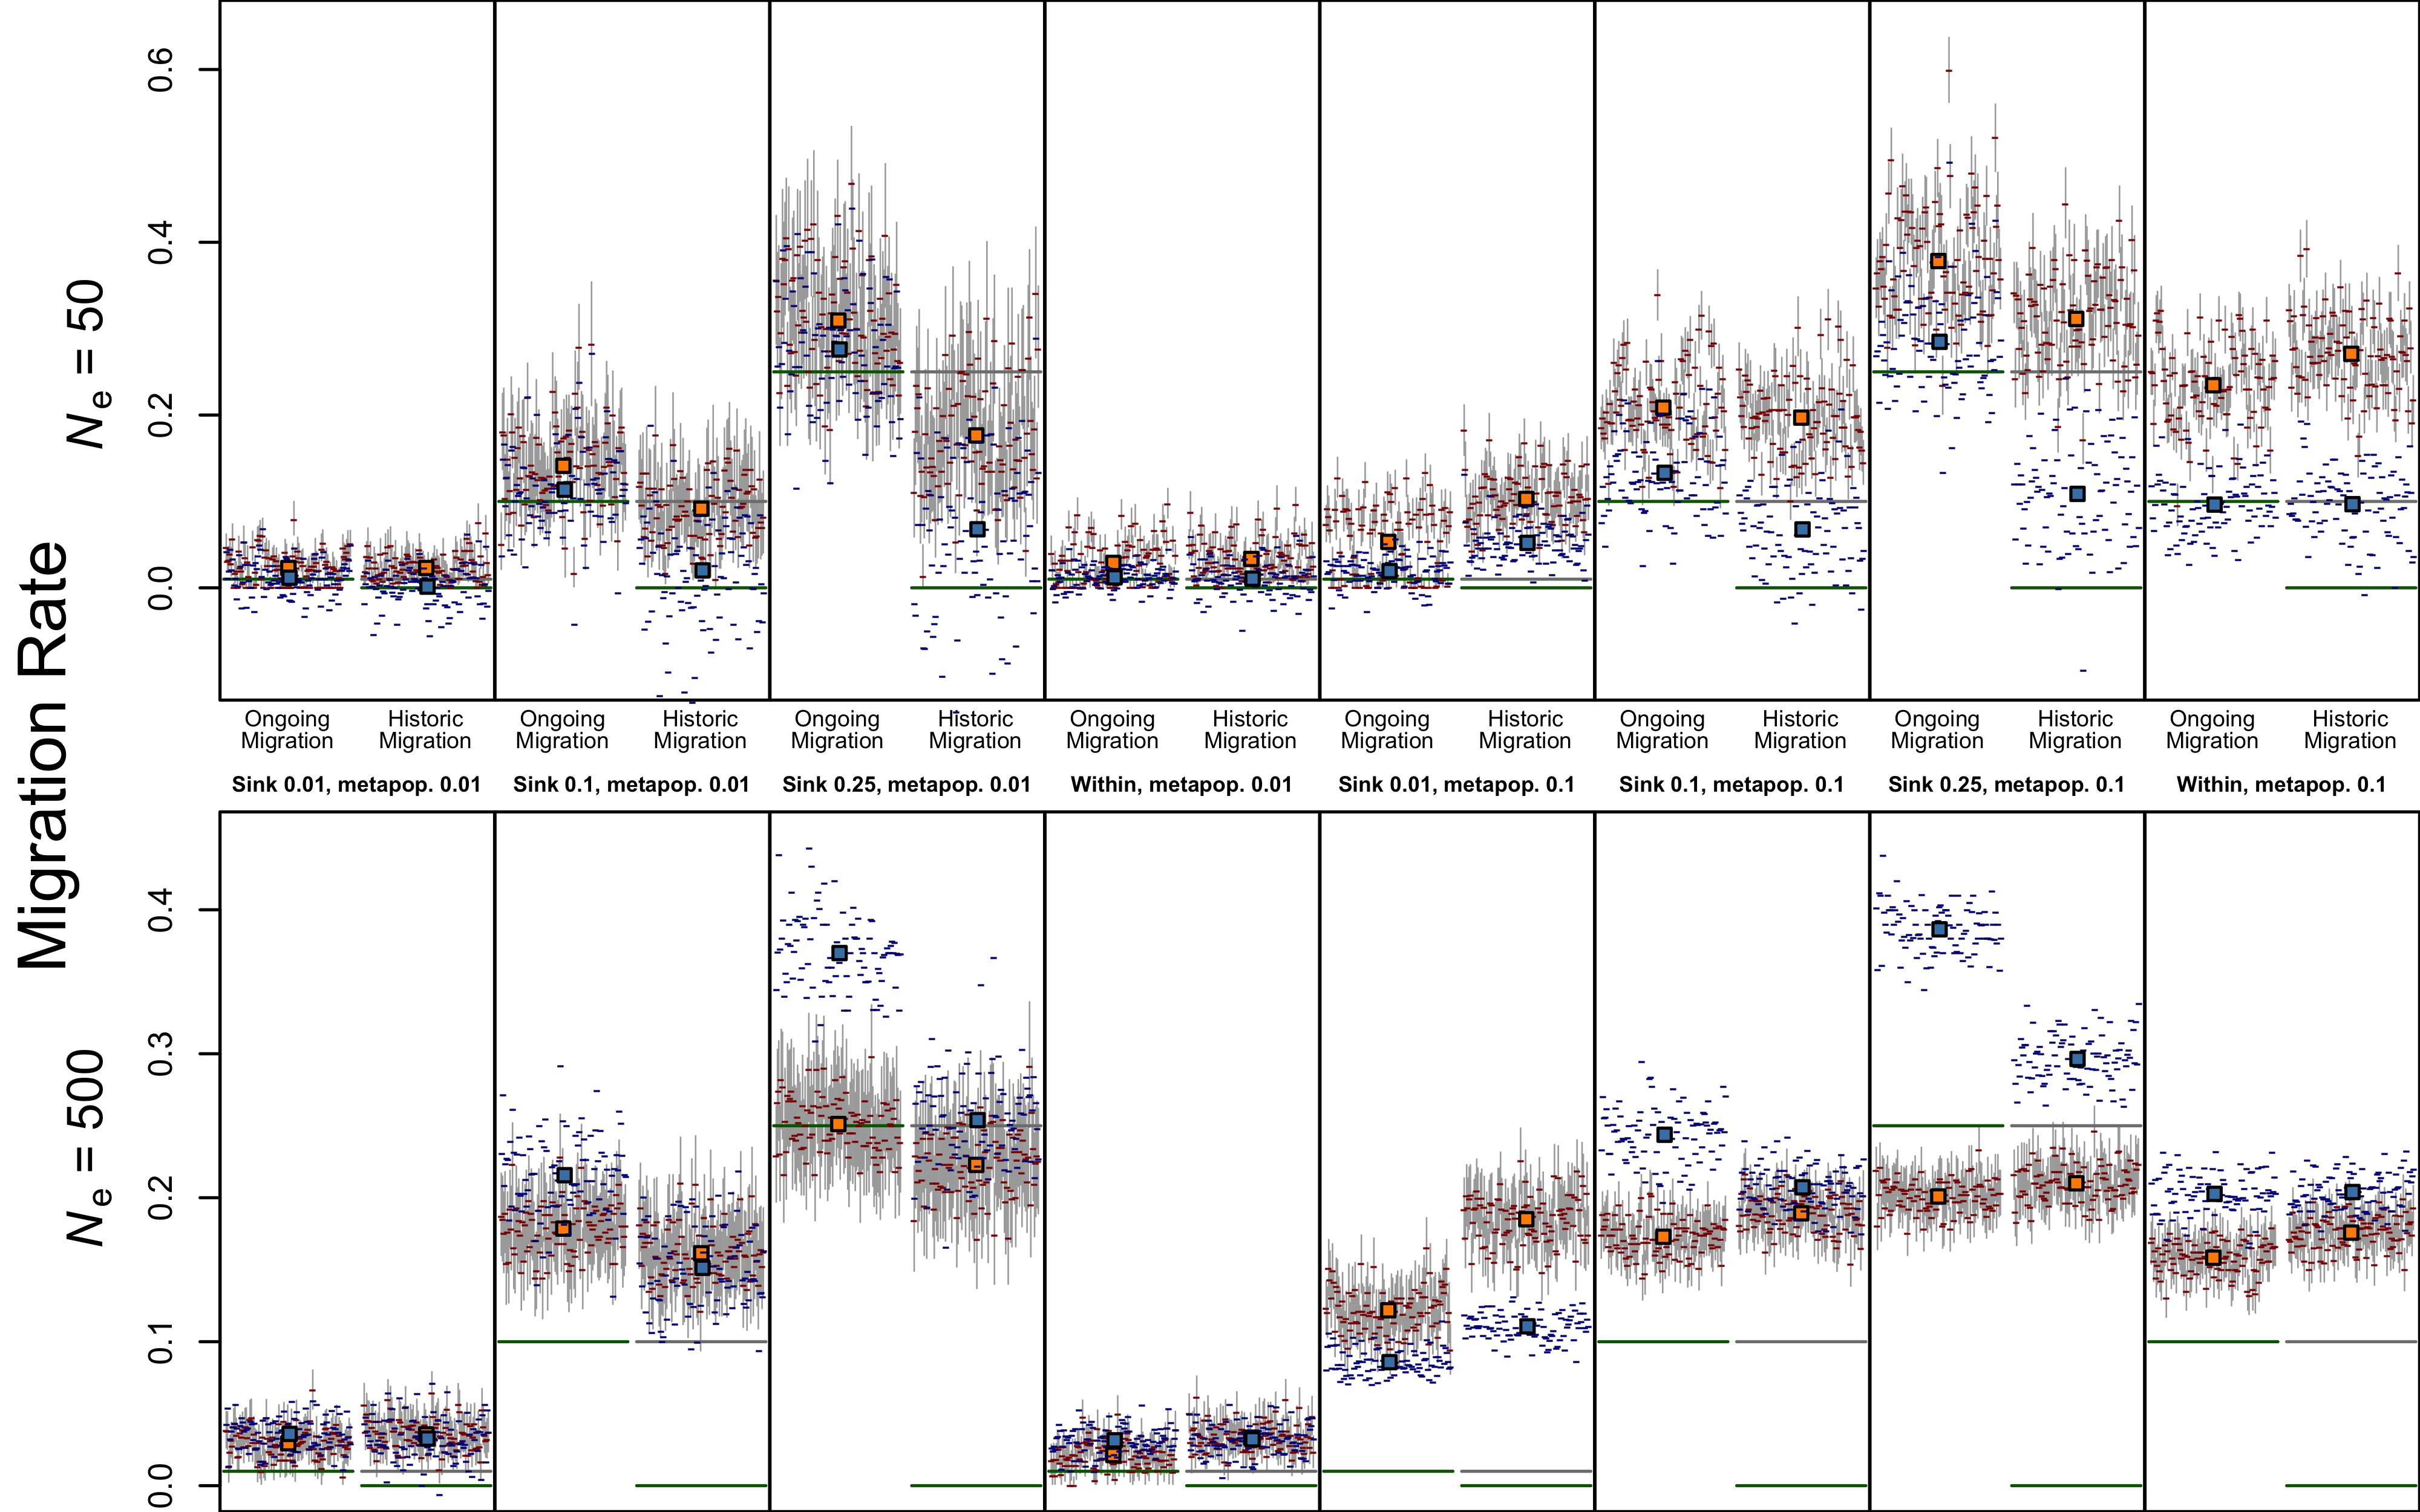
\includegraphics[width=0.8\linewidth]{Figures/SuppFigures/FigureS20__AssessMigrationRates.png}}
\caption[Comparing migration rates for ongoing versus historic migration scenarios.]{Comparing migration rates for ongoing versus historic migration scenarios estimated from \textsc{mlne}'s likelihood and moment methods. Green horizontal lines show the true migration rate, where the left half of each panel is the case where migration rate is constant and the right half of each panel shows the same populations except that migration stopped over the span of the temporal sampling. Therefore the true migration rate in the right half of each panel should reflect zero (green line) and the historic migration rate is shown by the horizontal gray line. Cases shown are sink populations and populations within the island model metapopulation where migration rates between the focal and source population are labeled in the center row and correspond to the panels both above and below each label. Population size of 50 is shown in the top row while 500 is shown in the bottom row.}
\label{fig:supp_compmig}
\end{figure}